% Options for packages loaded elsewhere
\PassOptionsToPackage{unicode}{hyperref}
\PassOptionsToPackage{hyphens}{url}
%
\documentclass[
]{article}
\usepackage{amsmath,amssymb}
\usepackage{iftex}
\ifPDFTeX
  \usepackage[T1]{fontenc}
  \usepackage[utf8]{inputenc}
  \usepackage{textcomp} % provide euro and other symbols
\else % if luatex or xetex
  \usepackage{unicode-math} % this also loads fontspec
  \defaultfontfeatures{Scale=MatchLowercase}
  \defaultfontfeatures[\rmfamily]{Ligatures=TeX,Scale=1}
\fi
\usepackage{lmodern}
\ifPDFTeX\else
  % xetex/luatex font selection
\fi
% Use upquote if available, for straight quotes in verbatim environments
\IfFileExists{upquote.sty}{\usepackage{upquote}}{}
\IfFileExists{microtype.sty}{% use microtype if available
  \usepackage[]{microtype}
  \UseMicrotypeSet[protrusion]{basicmath} % disable protrusion for tt fonts
}{}
\makeatletter
\@ifundefined{KOMAClassName}{% if non-KOMA class
  \IfFileExists{parskip.sty}{%
    \usepackage{parskip}
  }{% else
    \setlength{\parindent}{0pt}
    \setlength{\parskip}{6pt plus 2pt minus 1pt}}
}{% if KOMA class
  \KOMAoptions{parskip=half}}
\makeatother
\usepackage{xcolor}
\usepackage[margin=1in]{geometry}
\usepackage{graphicx}
\makeatletter
\def\maxwidth{\ifdim\Gin@nat@width>\linewidth\linewidth\else\Gin@nat@width\fi}
\def\maxheight{\ifdim\Gin@nat@height>\textheight\textheight\else\Gin@nat@height\fi}
\makeatother
% Scale images if necessary, so that they will not overflow the page
% margins by default, and it is still possible to overwrite the defaults
% using explicit options in \includegraphics[width, height, ...]{}
\setkeys{Gin}{width=\maxwidth,height=\maxheight,keepaspectratio}
% Set default figure placement to htbp
\makeatletter
\def\fps@figure{htbp}
\makeatother
\setlength{\emergencystretch}{3em} % prevent overfull lines
\providecommand{\tightlist}{%
  \setlength{\itemsep}{0pt}\setlength{\parskip}{0pt}}
\setcounter{secnumdepth}{-\maxdimen} % remove section numbering
\usepackage{booktabs}
\usepackage{longtable}
\usepackage{array}
\usepackage{multirow}
\usepackage{wrapfig}
\usepackage{float}
\usepackage{colortbl}
\usepackage{pdflscape}
\usepackage{tabu}
\usepackage{threeparttable}
\usepackage{threeparttablex}
\usepackage[normalem]{ulem}
\usepackage{makecell}
\usepackage{xcolor}
\ifLuaTeX
  \usepackage{selnolig}  % disable illegal ligatures
\fi
\IfFileExists{bookmark.sty}{\usepackage{bookmark}}{\usepackage{hyperref}}
\IfFileExists{xurl.sty}{\usepackage{xurl}}{} % add URL line breaks if available
\urlstyle{same}
\hypersetup{
  pdftitle={Using collaborative open science tools to improve engagement with the ecology of the Guana River Estuary},
  pdfauthor={Geraldine Klarenberg},
  hidelinks,
  pdfcreator={LaTeX via pandoc}}

\title{Using collaborative open science tools to improve engagement with
the ecology of the Guana River Estuary}
\author{Geraldine Klarenberg}
\date{2023-08-14}

\begin{document}
\maketitle

\hypertarget{project-team-geraldine-klarenberg-kristie-perez-nikki-dix-nia-morales-and-shirley-baker}{%
\subparagraph{\texorpdfstring{\emph{Project team: Geraldine Klarenberg,
Kristie Perez, Nikki Dix, Nia Morales, and Shirley
Baker}}{Project team: Geraldine Klarenberg, Kristie Perez, Nikki Dix, Nia Morales, and Shirley Baker}}\label{project-team-geraldine-klarenberg-kristie-perez-nikki-dix-nia-morales-and-shirley-baker}}

The University of Florida and Guana Tolomato Matanzas National Estuarine
Research Reserve (GTMNERR) are partnering with the local community and
broader science community to develop a web-based, public-facing,
interactive dashboard to provide access to Guana River Estuary (GRE)
datasets. The aim of this work is to support open science and to
increase diverse engagement with GRE within the GTMNERR by making the
data available interactively, using visualization tools.

To this end, the project team sought feedback from those who have been
involved with the GTMNERR to help them to better understand their needs.
This document summarizes the results of an online survey that was made
available via email, social media, and QR code.

\hypertarget{response-rate}{%
\subsubsection{1. Response rate}\label{response-rate}}

We received responses from 53 individuals. Out of these, .. were
unfinished. For the purposes of this report, we also took the unfinished
surveys into account.

.. respondents filled in the survey based on a link received via email,
.. via social media, .. via a QR code available at the GTMNERR Welcome
Center, and .. via a QR code available at the kiosk at the .. Dam.

\hypertarget{introductory-questions}{%
\subsubsection{2. Introductory questions}\label{introductory-questions}}

The survey asked respondents about their connection to the GTMNERR, how
often they engage with the GTMNERR, what data they would be interested
in, and whether or not they ever accessed data associated with the
GTMNERR.

\begin{verbatim}
## Warning in grid.Call(C_textBounds, as.graphicsAnnot(x$label), x$x, x$y, :
## conversion failure on '“Friends of GTM" member' in 'mbcsToSbcs': dot
## substituted for <e2>
\end{verbatim}

\begin{verbatim}
## Warning in grid.Call(C_textBounds, as.graphicsAnnot(x$label), x$x, x$y, :
## conversion failure on '“Friends of GTM" member' in 'mbcsToSbcs': dot
## substituted for <80>
\end{verbatim}

\begin{verbatim}
## Warning in grid.Call(C_textBounds, as.graphicsAnnot(x$label), x$x, x$y, :
## conversion failure on '“Friends of GTM" member' in 'mbcsToSbcs': dot
## substituted for <9c>
\end{verbatim}

\begin{verbatim}
## Warning in grid.Call(C_textBounds, as.graphicsAnnot(x$label), x$x, x$y, :
## conversion failure on '“Friends of GTM" member' in 'mbcsToSbcs': dot
## substituted for <e2>
\end{verbatim}

\begin{verbatim}
## Warning in grid.Call(C_textBounds, as.graphicsAnnot(x$label), x$x, x$y, :
## conversion failure on '“Friends of GTM" member' in 'mbcsToSbcs': dot
## substituted for <80>
\end{verbatim}

\begin{verbatim}
## Warning in grid.Call(C_textBounds, as.graphicsAnnot(x$label), x$x, x$y, :
## conversion failure on '“Friends of GTM" member' in 'mbcsToSbcs': dot
## substituted for <9c>
\end{verbatim}

\begin{verbatim}
## Warning in grid.Call(C_textBounds, as.graphicsAnnot(x$label), x$x, x$y, :
## conversion failure on '“Friends of GTM" member' in 'mbcsToSbcs': dot
## substituted for <e2>
\end{verbatim}

\begin{verbatim}
## Warning in grid.Call(C_textBounds, as.graphicsAnnot(x$label), x$x, x$y, :
## conversion failure on '“Friends of GTM" member' in 'mbcsToSbcs': dot
## substituted for <80>
\end{verbatim}

\begin{verbatim}
## Warning in grid.Call(C_textBounds, as.graphicsAnnot(x$label), x$x, x$y, :
## conversion failure on '“Friends of GTM" member' in 'mbcsToSbcs': dot
## substituted for <9c>
\end{verbatim}

\begin{verbatim}
## Warning in grid.Call(C_textBounds, as.graphicsAnnot(x$label), x$x, x$y, :
## conversion failure on '“Friends of GTM" member' in 'mbcsToSbcs': dot
## substituted for <e2>
\end{verbatim}

\begin{verbatim}
## Warning in grid.Call(C_textBounds, as.graphicsAnnot(x$label), x$x, x$y, :
## conversion failure on '“Friends of GTM" member' in 'mbcsToSbcs': dot
## substituted for <80>
\end{verbatim}

\begin{verbatim}
## Warning in grid.Call(C_textBounds, as.graphicsAnnot(x$label), x$x, x$y, :
## conversion failure on '“Friends of GTM" member' in 'mbcsToSbcs': dot
## substituted for <9c>
\end{verbatim}

\begin{verbatim}
## Warning in grid.Call(C_textBounds, as.graphicsAnnot(x$label), x$x, x$y, :
## conversion failure on '“Friends of GTM" member' in 'mbcsToSbcs': dot
## substituted for <e2>
\end{verbatim}

\begin{verbatim}
## Warning in grid.Call(C_textBounds, as.graphicsAnnot(x$label), x$x, x$y, :
## conversion failure on '“Friends of GTM" member' in 'mbcsToSbcs': dot
## substituted for <80>
\end{verbatim}

\begin{verbatim}
## Warning in grid.Call(C_textBounds, as.graphicsAnnot(x$label), x$x, x$y, :
## conversion failure on '“Friends of GTM" member' in 'mbcsToSbcs': dot
## substituted for <9c>
\end{verbatim}

\begin{verbatim}
## Warning in grid.Call(C_textBounds, as.graphicsAnnot(x$label), x$x, x$y, :
## conversion failure on '“Friends of GTM" member' in 'mbcsToSbcs': dot
## substituted for <e2>
\end{verbatim}

\begin{verbatim}
## Warning in grid.Call(C_textBounds, as.graphicsAnnot(x$label), x$x, x$y, :
## conversion failure on '“Friends of GTM" member' in 'mbcsToSbcs': dot
## substituted for <80>
\end{verbatim}

\begin{verbatim}
## Warning in grid.Call(C_textBounds, as.graphicsAnnot(x$label), x$x, x$y, :
## conversion failure on '“Friends of GTM" member' in 'mbcsToSbcs': dot
## substituted for <9c>
\end{verbatim}

\begin{verbatim}
## Warning in grid.Call(C_textBounds, as.graphicsAnnot(x$label), x$x, x$y, :
## conversion failure on '“Friends of GTM" member' in 'mbcsToSbcs': dot
## substituted for <e2>
\end{verbatim}

\begin{verbatim}
## Warning in grid.Call(C_textBounds, as.graphicsAnnot(x$label), x$x, x$y, :
## conversion failure on '“Friends of GTM" member' in 'mbcsToSbcs': dot
## substituted for <80>
\end{verbatim}

\begin{verbatim}
## Warning in grid.Call(C_textBounds, as.graphicsAnnot(x$label), x$x, x$y, :
## conversion failure on '“Friends of GTM" member' in 'mbcsToSbcs': dot
## substituted for <9c>
\end{verbatim}

\begin{verbatim}
## Warning in grid.Call(C_textBounds, as.graphicsAnnot(x$label), x$x, x$y, :
## conversion failure on '“Friends of GTM" member' in 'mbcsToSbcs': dot
## substituted for <e2>
\end{verbatim}

\begin{verbatim}
## Warning in grid.Call(C_textBounds, as.graphicsAnnot(x$label), x$x, x$y, :
## conversion failure on '“Friends of GTM" member' in 'mbcsToSbcs': dot
## substituted for <80>
\end{verbatim}

\begin{verbatim}
## Warning in grid.Call(C_textBounds, as.graphicsAnnot(x$label), x$x, x$y, :
## conversion failure on '“Friends of GTM" member' in 'mbcsToSbcs': dot
## substituted for <9c>
\end{verbatim}

\begin{verbatim}
## Warning in grid.Call(C_textBounds, as.graphicsAnnot(x$label), x$x, x$y, :
## conversion failure on '“Friends of GTM" member' in 'mbcsToSbcs': dot
## substituted for <e2>
\end{verbatim}

\begin{verbatim}
## Warning in grid.Call(C_textBounds, as.graphicsAnnot(x$label), x$x, x$y, :
## conversion failure on '“Friends of GTM" member' in 'mbcsToSbcs': dot
## substituted for <80>
\end{verbatim}

\begin{verbatim}
## Warning in grid.Call(C_textBounds, as.graphicsAnnot(x$label), x$x, x$y, :
## conversion failure on '“Friends of GTM" member' in 'mbcsToSbcs': dot
## substituted for <9c>
\end{verbatim}

\begin{verbatim}
## Warning in grid.Call(C_textBounds, as.graphicsAnnot(x$label), x$x, x$y, :
## conversion failure on '“Friends of GTM" member' in 'mbcsToSbcs': dot
## substituted for <e2>
\end{verbatim}

\begin{verbatim}
## Warning in grid.Call(C_textBounds, as.graphicsAnnot(x$label), x$x, x$y, :
## conversion failure on '“Friends of GTM" member' in 'mbcsToSbcs': dot
## substituted for <80>
\end{verbatim}

\begin{verbatim}
## Warning in grid.Call(C_textBounds, as.graphicsAnnot(x$label), x$x, x$y, :
## conversion failure on '“Friends of GTM" member' in 'mbcsToSbcs': dot
## substituted for <9c>
\end{verbatim}

\begin{verbatim}
## Warning in grid.Call(C_textBounds, as.graphicsAnnot(x$label), x$x, x$y, :
## conversion failure on '“Friends of GTM" member' in 'mbcsToSbcs': dot
## substituted for <e2>
\end{verbatim}

\begin{verbatim}
## Warning in grid.Call(C_textBounds, as.graphicsAnnot(x$label), x$x, x$y, :
## conversion failure on '“Friends of GTM" member' in 'mbcsToSbcs': dot
## substituted for <80>
\end{verbatim}

\begin{verbatim}
## Warning in grid.Call(C_textBounds, as.graphicsAnnot(x$label), x$x, x$y, :
## conversion failure on '“Friends of GTM" member' in 'mbcsToSbcs': dot
## substituted for <9c>
\end{verbatim}

\begin{verbatim}
## Warning in grid.Call(C_textBounds, as.graphicsAnnot(x$label), x$x, x$y, :
## conversion failure on '“Friends of GTM" member' in 'mbcsToSbcs': dot
## substituted for <e2>
\end{verbatim}

\begin{verbatim}
## Warning in grid.Call(C_textBounds, as.graphicsAnnot(x$label), x$x, x$y, :
## conversion failure on '“Friends of GTM" member' in 'mbcsToSbcs': dot
## substituted for <80>
\end{verbatim}

\begin{verbatim}
## Warning in grid.Call(C_textBounds, as.graphicsAnnot(x$label), x$x, x$y, :
## conversion failure on '“Friends of GTM" member' in 'mbcsToSbcs': dot
## substituted for <9c>
\end{verbatim}

\begin{verbatim}
## Warning in grid.Call(C_textBounds, as.graphicsAnnot(x$label), x$x, x$y, :
## conversion failure on '“Friends of GTM" member' in 'mbcsToSbcs': dot
## substituted for <e2>
\end{verbatim}

\begin{verbatim}
## Warning in grid.Call(C_textBounds, as.graphicsAnnot(x$label), x$x, x$y, :
## conversion failure on '“Friends of GTM" member' in 'mbcsToSbcs': dot
## substituted for <80>
\end{verbatim}

\begin{verbatim}
## Warning in grid.Call(C_textBounds, as.graphicsAnnot(x$label), x$x, x$y, :
## conversion failure on '“Friends of GTM" member' in 'mbcsToSbcs': dot
## substituted for <9c>
\end{verbatim}

\begin{verbatim}
## Warning in grid.Call(C_textBounds, as.graphicsAnnot(x$label), x$x, x$y, :
## conversion failure on '“Friends of GTM" member' in 'mbcsToSbcs': dot
## substituted for <e2>
\end{verbatim}

\begin{verbatim}
## Warning in grid.Call(C_textBounds, as.graphicsAnnot(x$label), x$x, x$y, :
## conversion failure on '“Friends of GTM" member' in 'mbcsToSbcs': dot
## substituted for <80>
\end{verbatim}

\begin{verbatim}
## Warning in grid.Call(C_textBounds, as.graphicsAnnot(x$label), x$x, x$y, :
## conversion failure on '“Friends of GTM" member' in 'mbcsToSbcs': dot
## substituted for <9c>
\end{verbatim}

\begin{verbatim}
## Warning in grid.Call(C_textBounds, as.graphicsAnnot(x$label), x$x, x$y, :
## conversion failure on '“Friends of GTM" member' in 'mbcsToSbcs': dot
## substituted for <e2>
\end{verbatim}

\begin{verbatim}
## Warning in grid.Call(C_textBounds, as.graphicsAnnot(x$label), x$x, x$y, :
## conversion failure on '“Friends of GTM" member' in 'mbcsToSbcs': dot
## substituted for <80>
\end{verbatim}

\begin{verbatim}
## Warning in grid.Call(C_textBounds, as.graphicsAnnot(x$label), x$x, x$y, :
## conversion failure on '“Friends of GTM" member' in 'mbcsToSbcs': dot
## substituted for <9c>
\end{verbatim}

\begin{verbatim}
## Warning in grid.Call.graphics(C_text, as.graphicsAnnot(x$label), x$x, x$y, :
## conversion failure on '“Friends of GTM" member' in 'mbcsToSbcs': dot
## substituted for <e2>
\end{verbatim}

\begin{verbatim}
## Warning in grid.Call.graphics(C_text, as.graphicsAnnot(x$label), x$x, x$y, :
## conversion failure on '“Friends of GTM" member' in 'mbcsToSbcs': dot
## substituted for <80>
\end{verbatim}

\begin{verbatim}
## Warning in grid.Call.graphics(C_text, as.graphicsAnnot(x$label), x$x, x$y, :
## conversion failure on '“Friends of GTM" member' in 'mbcsToSbcs': dot
## substituted for <9c>
\end{verbatim}

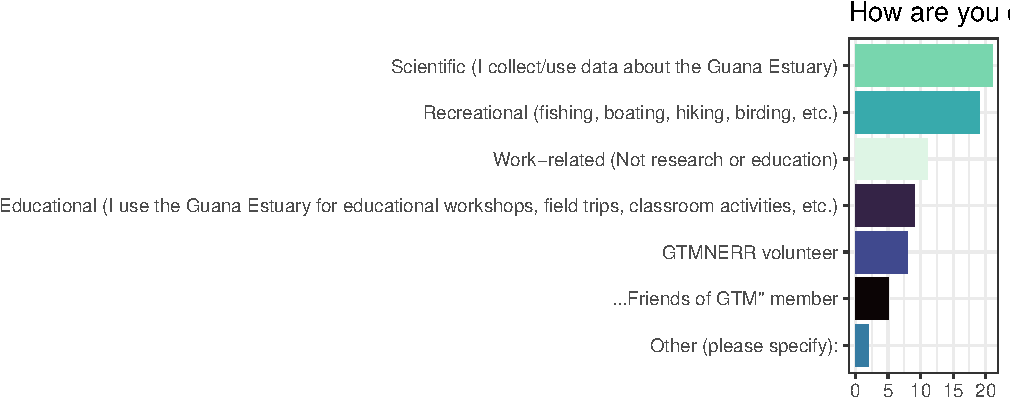
\includegraphics{survey_results_Aug2023_files/figure-latex/connected-1.pdf}

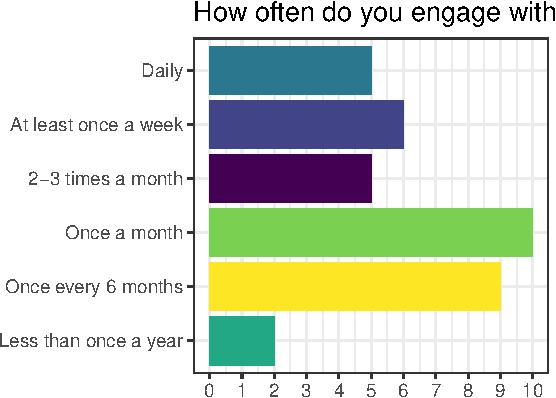
\includegraphics{survey_results_Aug2023_files/figure-latex/engage-1.pdf}

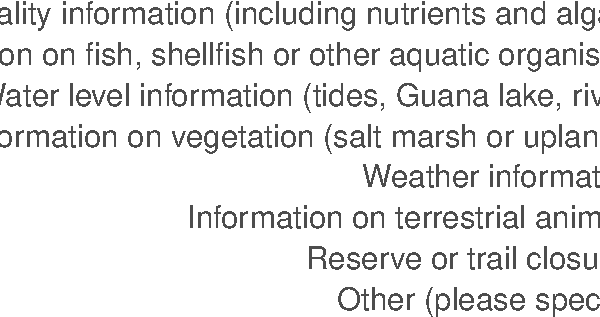
\includegraphics{survey_results_Aug2023_files/figure-latex/what_data-1.pdf}

Under ``Other'', the three types of data mentioned were: historical
maps, water fowl, and dam operations.

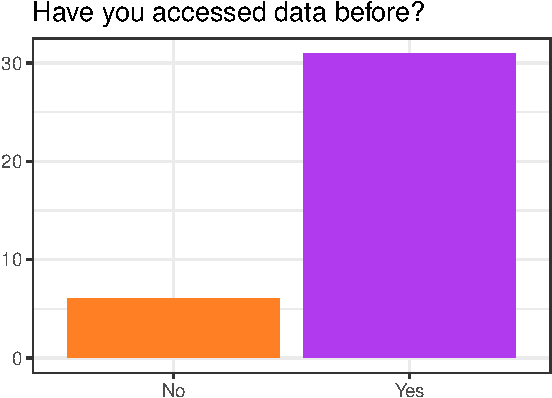
\includegraphics{survey_results_Aug2023_files/figure-latex/accessed_data-1.pdf}

\hypertarget{feedback-from-respondents-that-have-not-accessed-data-before}{%
\subsubsection{3. Feedback from respondents that have not accessed data
before}\label{feedback-from-respondents-that-have-not-accessed-data-before}}

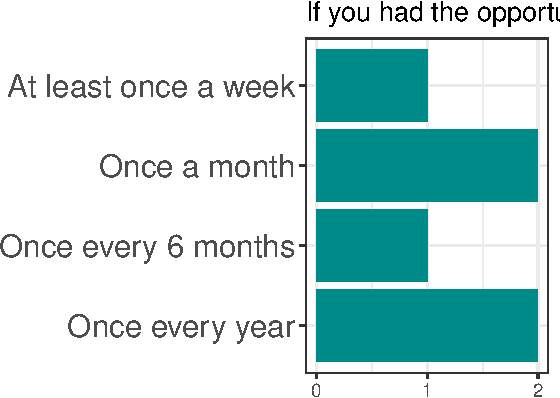
\includegraphics{survey_results_Aug2023_files/figure-latex/no_access_howoften-1.pdf}


\includegraphics{survey_results_Aug2023_files/figure-latex/no_access_what-1.pdf}

Under ``Other'', respondents listed: - environmental impacts, and -
resilience planning

\hypertarget{feedback-from-respondents-that-have-accessed-data-before}{%
\subsubsection{4. Feedback from respondents that have accessed data
before}\label{feedback-from-respondents-that-have-accessed-data-before}}

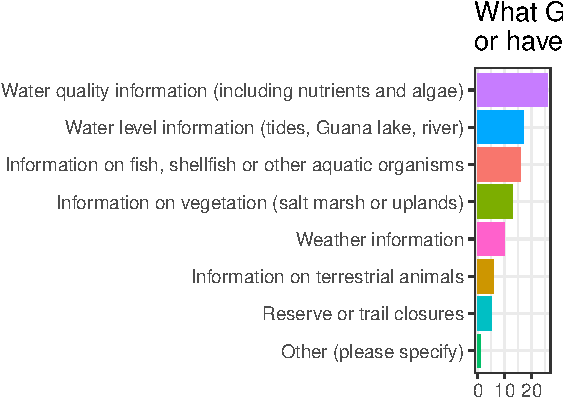
\includegraphics{survey_results_Aug2023_files/figure-latex/access_what-1.pdf}

\begin{table}
\centering
\begin{tabular}[t]{l|l|l|l|l|l|l|l}
\hline
q_text & Information on fish, shellfish or other aquatic organisms & Information on terrestrial animals & Information on vegetation (salt marsh or uplands) & Reserve or trail closures & Water level information (tides, Guana lake, river) & Water quality information (including nutrients and algae) & Weather information\\
\hline
\multicolumn{8}{l}{\textbf{How do you most frequently obtain or access these data?}}\\
\hline
\hspace{1em}Download from website (If so, what website?) & <span style="display: block; padding: 0 4px; border-radius: 4px; background-color: #71a63d">38</span> & <span style="display: block; padding: 0 4px; border-radius: 4px; background-color: #458b00">50</span> & <span style="display: block; padding: 0 4px; border-radius: 4px; background-color: #7cad4b">38</span> & <span style="display: block; padding: 0 4px; border-radius: 4px; background-color: #458b00">60</span> & <span style="display: block; padding: 0 4px; border-radius: 4px; background-color: #90ba67">35</span> & <span style="display: block; padding: 0 4px; border-radius: 4px; background-color: #9ac075">27</span> & <span style="display: block; padding: 0 4px; border-radius: 4px; background-color: #458b00">70</span>\\
\hline
\hspace{1em}Other (please specify) & <span style="display: block; padding: 0 4px; border-radius: 4px; background-color: #d2e3c1">12</span> & <span style="display: block; padding: 0 4px; border-radius: 4px; background-color: #bfd7a8">17</span> & <span style="display: block; padding: 0 4px; border-radius: 4px; background-color: #cbdeb8">15</span> & <span style="display: block; padding: 0 4px; border-radius: 4px; background-color: #ffffff">0</span> & <span style="display: block; padding: 0 4px; border-radius: 4px; background-color: #b3cf97">24</span> & <span style="display: block; padding: 0 4px; border-radius: 4px; background-color: #a9c989">23</span> & <span style="display: block; padding: 0 4px; border-radius: 4px; background-color: #afcd91">30</span>\\
\hline
\hspace{1em}Request from a GTMNERR staff member by email & <span style="display: block; padding: 0 4px; border-radius: 4px; background-color: #458b00">50</span> & <span style="display: block; padding: 0 4px; border-radius: 4px; background-color: #84b256">33</span> & <span style="display: block; padding: 0 4px; border-radius: 4px; background-color: #609c25">46</span> & <span style="display: block; padding: 0 4px; border-radius: 4px; background-color: #c1d8aa">20</span> & <span style="display: block; padding: 0 4px; border-radius: 4px; background-color: #7dae4d">41</span> & <span style="display: block; padding: 0 4px; border-radius: 4px; background-color: #458b00">50</span> & <span style="display: block; padding: 0 4px; border-radius: 4px; background-color: #ffffff">0</span>\\
\hline
\hspace{1em}Pick-up paper copy in person & <span style="display: block; padding: 0 4px; border-radius: 4px; background-color: #ffffff">0</span> & <span style="display: block; padding: 0 4px; border-radius: 4px; background-color: #ffffff">0</span> & <span style="display: block; padding: 0 4px; border-radius: 4px; background-color: #ffffff">0</span> & <span style="display: block; padding: 0 4px; border-radius: 4px; background-color: #c1d8aa">20</span> & <span style="display: block; padding: 0 4px; border-radius: 4px; background-color: #ffffff">0</span> & <span style="display: block; padding: 0 4px; border-radius: 4px; background-color: #ffffff">0</span> & <span style="display: block; padding: 0 4px; border-radius: 4px; background-color: #ffffff">0</span>\\
\hline
\multicolumn{8}{l}{\textbf{What are the advantages of this primary method of accessing or obtaining these data?}}\\
\hline
\hspace{1em}Data is received quickly after request & <span style="display: block; padding: 0 4px; border-radius: 4px; background-color: #b8d29e">19</span> & <span style="display: block; padding: 0 4px; border-radius: 4px; background-color: #ffffff">0</span> & <span style="display: block; padding: 0 4px; border-radius: 4px; background-color: #d2e3c1">13</span> & <span style="display: block; padding: 0 4px; border-radius: 4px; background-color: #b1ce94">25</span> & <span style="display: block; padding: 0 4px; border-radius: 4px; background-color: #c9ddb5">17</span> & <span style="display: block; padding: 0 4px; border-radius: 4px; background-color: #bfd7a8">17</span> & <span style="display: block; padding: 0 4px; border-radius: 4px; background-color: #e1ecd6">11</span>\\
\hline
\hspace{1em}Easy/convenient to access & <span style="display: block; padding: 0 4px; border-radius: 4px; background-color: #84b256">33</span> & <span style="display: block; padding: 0 4px; border-radius: 4px; background-color: #5b981e">44</span> & <span style="display: block; padding: 0 4px; border-radius: 4px; background-color: #6aa233">43</span> & <span style="display: block; padding: 0 4px; border-radius: 4px; background-color: #b1ce94">25</span> & <span style="display: block; padding: 0 4px; border-radius: 4px; background-color: #87b45a">38</span> & <span style="display: block; padding: 0 4px; border-radius: 4px; background-color: #7cad4c">35</span> & <span style="display: block; padding: 0 4px; border-radius: 4px; background-color: #8fb966">42</span>\\
\hline
\hspace{1em}Other (please specify) & <span style="display: block; padding: 0 4px; border-radius: 4px; background-color: #e1ecd6">8</span> & <span style="display: block; padding: 0 4px; border-radius: 4px; background-color: #ffffff">0</span> & <span style="display: block; padding: 0 4px; border-radius: 4px; background-color: #ffffff">0</span> & <span style="display: block; padding: 0 4px; border-radius: 4px; background-color: #e6efdd">8</span> & <span style="display: block; padding: 0 4px; border-radius: 4px; background-color: #ffffff">0</span> & <span style="display: block; padding: 0 4px; border-radius: 4px; background-color: #f7faf4">2</span> & <span style="display: block; padding: 0 4px; border-radius: 4px; background-color: #ffffff">0</span>\\
\hline
\hspace{1em}Requesting the data is quick & <span style="display: block; padding: 0 4px; border-radius: 4px; background-color: #d6e5c6">11</span> & <span style="display: block; padding: 0 4px; border-radius: 4px; background-color: #d6e5c6">11</span> & <span style="display: block; padding: 0 4px; border-radius: 4px; background-color: #d2e3c1">13</span> & <span style="display: block; padding: 0 4px; border-radius: 4px; background-color: #cadeb6">17</span> & <span style="display: block; padding: 0 4px; border-radius: 4px; background-color: #d2e3c2">14</span> & <span style="display: block; padding: 0 4px; border-radius: 4px; background-color: #bfd7a8">17</span> & <span style="display: block; padding: 0 4px; border-radius: 4px; background-color: #d4e4c4">16</span>\\
\hline
\hspace{1em}The format the data are delivered / accessed in is useful & <span style="display: block; padding: 0 4px; border-radius: 4px; background-color: #96be70">28</span> & <span style="display: block; padding: 0 4px; border-radius: 4px; background-color: #84b256">33</span> & <span style="display: block; padding: 0 4px; border-radius: 4px; background-color: #b3cf97">22</span> & <span style="display: block; padding: 0 4px; border-radius: 4px; background-color: #cadeb6">17</span> & <span style="display: block; padding: 0 4px; border-radius: 4px; background-color: #b3cf97">24</span> & <span style="display: block; padding: 0 4px; border-radius: 4px; background-color: #9ec27a">26</span> & <span style="display: block; padding: 0 4px; border-radius: 4px; background-color: #c7dcb2">21</span>\\
\hline
\hspace{1em}There are no advantages & <span style="display: block; padding: 0 4px; border-radius: 4px; background-color: #ffffff">0</span> & <span style="display: block; padding: 0 4px; border-radius: 4px; background-color: #d6e5c6">11</span> & <span style="display: block; padding: 0 4px; border-radius: 4px; background-color: #e0ebd4">9</span> & <span style="display: block; padding: 0 4px; border-radius: 4px; background-color: #e6efdd">8</span> & <span style="display: block; padding: 0 4px; border-radius: 4px; background-color: #e8f1e0">7</span> & <span style="display: block; padding: 0 4px; border-radius: 4px; background-color: #f7faf4">2</span> & <span style="display: block; padding: 0 4px; border-radius: 4px; background-color: #e1ecd6">11</span>\\
\hline
\multicolumn{8}{l}{\textbf{What are the disadvantages of the primary method of accessing or obtaining these data?}}\\
\hline
\hspace{1em}Difficult/Complicated to access & <span style="display: block; padding: 0 4px; border-radius: 4px; background-color: #d6e5c6">11</span> & <span style="display: block; padding: 0 4px; border-radius: 4px; background-color: #d6e5c6">11</span> & <span style="display: block; padding: 0 4px; border-radius: 4px; background-color: #e6efdd">7</span> & <span style="display: block; padding: 0 4px; border-radius: 4px; background-color: #cadeb6">17</span> & <span style="display: block; padding: 0 4px; border-radius: 4px; background-color: #ecf3e5">6</span> & <span style="display: block; padding: 0 4px; border-radius: 4px; background-color: #d9e7cc">10</span> & <span style="display: block; padding: 0 4px; border-radius: 4px; background-color: #d7e6c8">15</span>\\
\hline
\hspace{1em}Other (please specify) & <span style="display: block; padding: 0 4px; border-radius: 4px; background-color: #b0ce93">21</span> & <span style="display: block; padding: 0 4px; border-radius: 4px; background-color: #84b256">33</span> & <span style="display: block; padding: 0 4px; border-radius: 4px; background-color: #bad4a0">20</span> & <span style="display: block; padding: 0 4px; border-radius: 4px; background-color: #98bf72">33</span> & <span style="display: block; padding: 0 4px; border-radius: 4px; background-color: #b9d39f">22</span> & <span style="display: block; padding: 0 4px; border-radius: 4px; background-color: #93bb6b">29</span> & <span style="display: block; padding: 0 4px; border-radius: 4px; background-color: #c1d8ab">23</span>\\
\hline
\hspace{1em}Slow to receive & <span style="display: block; padding: 0 4px; border-radius: 4px; background-color: #ecf3e5">5</span> & <span style="display: block; padding: 0 4px; border-radius: 4px; background-color: #d6e5c6">11</span> & <span style="display: block; padding: 0 4px; border-radius: 4px; background-color: #e6efdd">7</span> & <span style="display: block; padding: 0 4px; border-radius: 4px; background-color: #ffffff">0</span> & <span style="display: block; padding: 0 4px; border-radius: 4px; background-color: #dce9cf">11</span> & <span style="display: block; padding: 0 4px; border-radius: 4px; background-color: #f3f8ef">3</span> & <span style="display: block; padding: 0 4px; border-radius: 4px; background-color: #d7e6c8">15</span>\\
\hline
\hspace{1em}The format the data are delivered / accessed in is not user-friendly & <span style="display: block; padding: 0 4px; border-radius: 4px; background-color: #d6e5c6">11</span> & <span style="display: block; padding: 0 4px; border-radius: 4px; background-color: #ffffff">0</span> & <span style="display: block; padding: 0 4px; border-radius: 4px; background-color: #d2e3c1">13</span> & <span style="display: block; padding: 0 4px; border-radius: 4px; background-color: #ffffff">0</span> & <span style="display: block; padding: 0 4px; border-radius: 4px; background-color: #dce9cf">11</span> & <span style="display: block; padding: 0 4px; border-radius: 4px; background-color: #d9e7cc">10</span> & <span style="display: block; padding: 0 4px; border-radius: 4px; background-color: #e9f1e1">8</span>\\
\hline
\hspace{1em}There are no disadvantages & <span style="display: block; padding: 0 4px; border-radius: 4px; background-color: #629d28">42</span> & <span style="display: block; padding: 0 4px; border-radius: 4px; background-color: #d6e5c6">11</span> & <span style="display: block; padding: 0 4px; border-radius: 4px; background-color: #75a942">40</span> & <span style="display: block; padding: 0 4px; border-radius: 4px; background-color: #649e2a">50</span> & <span style="display: block; padding: 0 4px; border-radius: 4px; background-color: #84b256">39</span> & <span style="display: block; padding: 0 4px; border-radius: 4px; background-color: #7cad4c">35</span> & <span style="display: block; padding: 0 4px; border-radius: 4px; background-color: #accb8e">31</span>\\
\hline
\hspace{1em}Time consuming to request & <span style="display: block; padding: 0 4px; border-radius: 4px; background-color: #d6e5c6">11</span> & <span style="display: block; padding: 0 4px; border-radius: 4px; background-color: #84b256">33</span> & <span style="display: block; padding: 0 4px; border-radius: 4px; background-color: #d2e3c1">13</span> & <span style="display: block; padding: 0 4px; border-radius: 4px; background-color: #ffffff">0</span> & <span style="display: block; padding: 0 4px; border-radius: 4px; background-color: #dce9cf">11</span> & <span style="display: block; padding: 0 4px; border-radius: 4px; background-color: #cee0bc">13</span> & <span style="display: block; padding: 0 4px; border-radius: 4px; background-color: #e9f1e1">8</span>\\
\hline
\multicolumn{8}{l}{\textbf{How often do/did you access or obtain these data?}}\\
\hline
\hspace{1em}2-3 times a month & <span style="display: block; padding: 0 4px; border-radius: 4px; background-color: #a2c57f">25</span> & <span style="display: block; padding: 0 4px; border-radius: 4px; background-color: #bfd7a8">17</span> & <span style="display: block; padding: 0 4px; border-radius: 4px; background-color: #afcd92">23</span> & <span style="display: block; padding: 0 4px; border-radius: 4px; background-color: #ffffff">0</span> & <span style="display: block; padding: 0 4px; border-radius: 4px; background-color: #ffffff">0</span> & <span style="display: block; padding: 0 4px; border-radius: 4px; background-color: #e1ecd6">8</span> & <span style="display: block; padding: 0 4px; border-radius: 4px; background-color: #ffffff">0</span>\\
\hline
\hspace{1em}Daily & <span style="display: block; padding: 0 4px; border-radius: 4px; background-color: #e8f1e0">6</span> & <span style="display: block; padding: 0 4px; border-radius: 4px; background-color: #bfd7a8">17</span> & <span style="display: block; padding: 0 4px; border-radius: 4px; background-color: #e3edd9">8</span> & <span style="display: block; padding: 0 4px; border-radius: 4px; background-color: #c1d8aa">20</span> & <span style="display: block; padding: 0 4px; border-radius: 4px; background-color: #d9e7cb">12</span> & <span style="display: block; padding: 0 4px; border-radius: 4px; background-color: #ffffff">0</span> & <span style="display: block; padding: 0 4px; border-radius: 4px; background-color: #e4eeda">10</span>\\
\hline
\hspace{1em}Less than once a year & <span style="display: block; padding: 0 4px; border-radius: 4px; background-color: #b8d29e">19</span> & <span style="display: block; padding: 0 4px; border-radius: 4px; background-color: #ffffff">0</span> & <span style="display: block; padding: 0 4px; border-radius: 4px; background-color: #cbdeb8">15</span> & <span style="display: block; padding: 0 4px; border-radius: 4px; background-color: #ffffff">0</span> & <span style="display: block; padding: 0 4px; border-radius: 4px; background-color: #b3cf97">24</span> & <span style="display: block; padding: 0 4px; border-radius: 4px; background-color: #b8d29e">19</span> & <span style="display: block; padding: 0 4px; border-radius: 4px; background-color: #ffffff">0</span>\\
\hline
\hspace{1em}Once a month & <span style="display: block; padding: 0 4px; border-radius: 4px; background-color: #b8d29e">19</span> & <span style="display: block; padding: 0 4px; border-radius: 4px; background-color: #84b256">33</span> & <span style="display: block; padding: 0 4px; border-radius: 4px; background-color: #afcd92">23</span> & <span style="display: block; padding: 0 4px; border-radius: 4px; background-color: #c1d8aa">20</span> & <span style="display: block; padding: 0 4px; border-radius: 4px; background-color: #c6dbb1">18</span> & <span style="display: block; padding: 0 4px; border-radius: 4px; background-color: #b8d29e">19</span> & <span style="display: block; padding: 0 4px; border-radius: 4px; background-color: #5f9b24">60</span>\\
\hline
\hspace{1em}Once every 6 months & <span style="display: block; padding: 0 4px; border-radius: 4px; background-color: #8bb760">31</span> & <span style="display: block; padding: 0 4px; border-radius: 4px; background-color: #84b256">33</span> & <span style="display: block; padding: 0 4px; border-radius: 4px; background-color: #e3edd9">8</span> & <span style="display: block; padding: 0 4px; border-radius: 4px; background-color: #83b155">40</span> & <span style="display: block; padding: 0 4px; border-radius: 4px; background-color: #a3c581">29</span> & <span style="display: block; padding: 0 4px; border-radius: 4px; background-color: #a9c989">23</span> & <span style="display: block; padding: 0 4px; border-radius: 4px; background-color: #c9ddb6">20</span>\\
\hline
\hspace{1em}Once every year & <span style="display: block; padding: 0 4px; border-radius: 4px; background-color: #ffffff">0</span> & <span style="display: block; padding: 0 4px; border-radius: 4px; background-color: #ffffff">0</span> & <span style="display: block; padding: 0 4px; border-radius: 4px; background-color: #afcd92">23</span> & <span style="display: block; padding: 0 4px; border-radius: 4px; background-color: #c1d8aa">20</span> & <span style="display: block; padding: 0 4px; border-radius: 4px; background-color: #ffffff">0</span> & <span style="display: block; padding: 0 4px; border-radius: 4px; background-color: #9ac075">27</span> & <span style="display: block; padding: 0 4px; border-radius: 4px; background-color: #e4eeda">10</span>\\
\hline
\hspace{1em}At least once a week & <span style="display: block; padding: 0 4px; border-radius: 4px; background-color: #ffffff">0</span> & <span style="display: block; padding: 0 4px; border-radius: 4px; background-color: #ffffff">0</span> & <span style="display: block; padding: 0 4px; border-radius: 4px; background-color: #ffffff">0</span> & <span style="display: block; padding: 0 4px; border-radius: 4px; background-color: #ffffff">0</span> & <span style="display: block; padding: 0 4px; border-radius: 4px; background-color: #c6dbb1">18</span> & <span style="display: block; padding: 0 4px; border-radius: 4px; background-color: #f0f5ea">4</span> & <span style="display: block; padding: 0 4px; border-radius: 4px; background-color: #ffffff">0</span>\\
\hline
\multicolumn{8}{l}{\textbf{What do you typically use these data for?}}\\
\hline
\hspace{1em}Decision making (for recreational/educational/scientific visits) & <span style="display: block; padding: 0 4px; border-radius: 4px; background-color: #d6e5c6">11</span> & <span style="display: block; padding: 0 4px; border-radius: 4px; background-color: #bcd5a3">18</span> & <span style="display: block; padding: 0 4px; border-radius: 4px; background-color: #d2e3c1">13</span> & <span style="display: block; padding: 0 4px; border-radius: 4px; background-color: #bad4a1">22</span> & <span style="display: block; padding: 0 4px; border-radius: 4px; background-color: #c3d9ac">19</span> & <span style="display: block; padding: 0 4px; border-radius: 4px; background-color: #cadeb7">14</span> & <span style="display: block; padding: 0 4px; border-radius: 4px; background-color: #c4daae">22</span>\\
\hline
\hspace{1em}Educational purposes & <span style="display: block; padding: 0 4px; border-radius: 4px; background-color: #adcb8e">22</span> & <span style="display: block; padding: 0 4px; border-radius: 4px; background-color: #9ac075">27</span> & <span style="display: block; padding: 0 4px; border-radius: 4px; background-color: #b3cf97">22</span> & <span style="display: block; padding: 0 4px; border-radius: 4px; background-color: #98bf72">33</span> & <span style="display: block; padding: 0 4px; border-radius: 4px; background-color: #cfe1be">15</span> & <span style="display: block; padding: 0 4px; border-radius: 4px; background-color: #cadeb7">14</span> & <span style="display: block; padding: 0 4px; border-radius: 4px; background-color: #d1e2c1">17</span>\\
\hline
\hspace{1em}Monitoring & <span style="display: block; padding: 0 4px; border-radius: 4px; background-color: #c7dcb2">15</span> & <span style="display: block; padding: 0 4px; border-radius: 4px; background-color: #bcd5a3">18</span> & <span style="display: block; padding: 0 4px; border-radius: 4px; background-color: #d2e3c1">13</span> & <span style="display: block; padding: 0 4px; border-radius: 4px; background-color: #dce9d0">11</span> & <span style="display: block; padding: 0 4px; border-radius: 4px; background-color: #e8f1e0">7</span> & <span style="display: block; padding: 0 4px; border-radius: 4px; background-color: #cadeb7">14</span> & <span style="display: block; padding: 0 4px; border-radius: 4px; background-color: #ffffff">0</span>\\
\hline
\hspace{1em}Research & <span style="display: block; padding: 0 4px; border-radius: 4px; background-color: #75a942">37</span> & <span style="display: block; padding: 0 4px; border-radius: 4px; background-color: #ddead1">9</span> & <span style="display: block; padding: 0 4px; border-radius: 4px; background-color: #a5c784">26</span> & <span style="display: block; padding: 0 4px; border-radius: 4px; background-color: #dce9d0">11</span> & <span style="display: block; padding: 0 4px; border-radius: 4px; background-color: #a0c47d">30</span> & <span style="display: block; padding: 0 4px; border-radius: 4px; background-color: #84b256">33</span> & <span style="display: block; padding: 0 4px; border-radius: 4px; background-color: #b4d099">28</span>\\
\hline
\hspace{1em}Work-related purposes (not research or education) & <span style="display: block; padding: 0 4px; border-radius: 4px; background-color: #c7dcb2">15</span> & <span style="display: block; padding: 0 4px; border-radius: 4px; background-color: #bcd5a3">18</span> & <span style="display: block; padding: 0 4px; border-radius: 4px; background-color: #c4daae">17</span> & <span style="display: block; padding: 0 4px; border-radius: 4px; background-color: #dce9d0">11</span> & <span style="display: block; padding: 0 4px; border-radius: 4px; background-color: #b9d39f">22</span> & <span style="display: block; padding: 0 4px; border-radius: 4px; background-color: #b8d29e">19</span> & <span style="display: block; padding: 0 4px; border-radius: 4px; background-color: #c4daae">22</span>\\
\hline
\hspace{1em}Other (please specify) & <span style="display: block; padding: 0 4px; border-radius: 4px; background-color: #ffffff">0</span> & <span style="display: block; padding: 0 4px; border-radius: 4px; background-color: #ddead1">9</span> & <span style="display: block; padding: 0 4px; border-radius: 4px; background-color: #e0ebd4">9</span> & <span style="display: block; padding: 0 4px; border-radius: 4px; background-color: #dce9d0">11</span> & <span style="display: block; padding: 0 4px; border-radius: 4px; background-color: #e8f1e0">7</span> & <span style="display: block; padding: 0 4px; border-radius: 4px; background-color: #ecf3e5">5</span> & <span style="display: block; padding: 0 4px; border-radius: 4px; background-color: #e1ecd6">11</span>\\
\hline
\multicolumn{8}{l}{\textbf{How well do these data generally satisfy your need(s)?}}\\
\hline
\hspace{1em}Extremely well & <span style="display: block; padding: 0 4px; border-radius: 4px; background-color: #e8f1e0">6</span> & <span style="display: block; padding: 0 4px; border-radius: 4px; background-color: #bfd7a8">17</span> & <span style="display: block; padding: 0 4px; border-radius: 4px; background-color: #ffffff">0</span> & <span style="display: block; padding: 0 4px; border-radius: 4px; background-color: #c1d8aa">20</span> & <span style="display: block; padding: 0 4px; border-radius: 4px; background-color: #ecf3e5">6</span> & <span style="display: block; padding: 0 4px; border-radius: 4px; background-color: #f0f5ea">4</span> & <span style="display: block; padding: 0 4px; border-radius: 4px; background-color: #e4eeda">10</span>\\
\hline
\hspace{1em}Moderately well & <span style="display: block; padding: 0 4px; border-radius: 4px; background-color: #5b981e">44</span> & <span style="display: block; padding: 0 4px; border-radius: 4px; background-color: #84b256">33</span> & <span style="display: block; padding: 0 4px; border-radius: 4px; background-color: #609c25">46</span> & <span style="display: block; padding: 0 4px; border-radius: 4px; background-color: #c1d8aa">20</span> & <span style="display: block; padding: 0 4px; border-radius: 4px; background-color: #458b00">59</span> & <span style="display: block; padding: 0 4px; border-radius: 4px; background-color: #7cad4c">35</span> & <span style="display: block; padding: 0 4px; border-radius: 4px; background-color: #afcd91">30</span>\\
\hline
\hspace{1em}Slightly well & <span style="display: block; padding: 0 4px; border-radius: 4px; background-color: #d2e3c1">12</span> & <span style="display: block; padding: 0 4px; border-radius: 4px; background-color: #84b256">33</span> & <span style="display: block; padding: 0 4px; border-radius: 4px; background-color: #ffffff">0</span> & <span style="display: block; padding: 0 4px; border-radius: 4px; background-color: #ffffff">0</span> & <span style="display: block; padding: 0 4px; border-radius: 4px; background-color: #ecf3e5">6</span> & <span style="display: block; padding: 0 4px; border-radius: 4px; background-color: #c7dcb2">15</span> & <span style="display: block; padding: 0 4px; border-radius: 4px; background-color: #c9ddb6">20</span>\\
\hline
\hspace{1em}Very well & <span style="display: block; padding: 0 4px; border-radius: 4px; background-color: #71a63d">38</span> & <span style="display: block; padding: 0 4px; border-radius: 4px; background-color: #bfd7a8">17</span> & <span style="display: block; padding: 0 4px; border-radius: 4px; background-color: #458b00">54</span> & <span style="display: block; padding: 0 4px; border-radius: 4px; background-color: #458b00">60</span> & <span style="display: block; padding: 0 4px; border-radius: 4px; background-color: #a3c581">29</span> & <span style="display: block; padding: 0 4px; border-radius: 4px; background-color: #539414">46</span> & <span style="display: block; padding: 0 4px; border-radius: 4px; background-color: #94bc6d">40</span>\\
\hline
\end{tabular}
\end{table}

Add info on Other

\hypertarget{dashboard-preferences}{%
\subsubsection{5. Dashboard preferences}\label{dashboard-preferences}}

The survey asked respondents about their preferences regarding dashboard
features (type and format of information, data delivery mode) and how
they would access the dashboard.

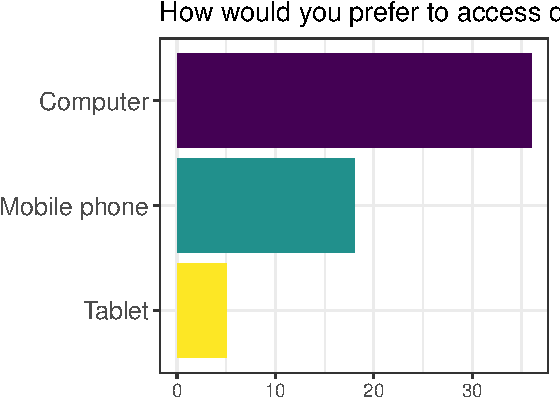
\includegraphics{survey_results_Aug2023_files/figure-latex/dash_how-1.pdf}

\begin{center}\rule{0.5\linewidth}{0.5pt}\end{center}

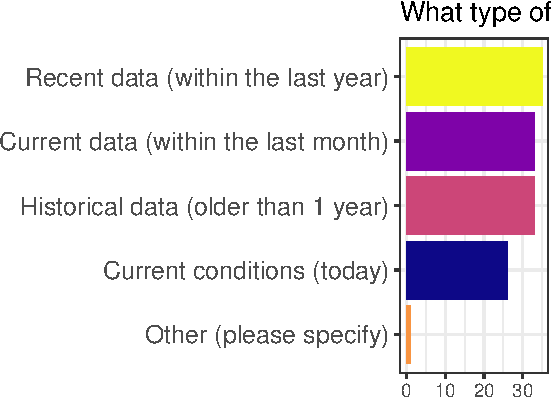
\includegraphics{survey_results_Aug2023_files/figure-latex/dash_type-1.pdf}

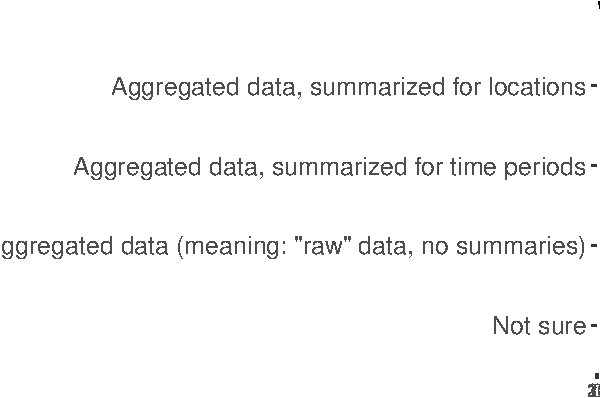
\includegraphics{survey_results_Aug2023_files/figure-latex/dash_form-1.pdf}

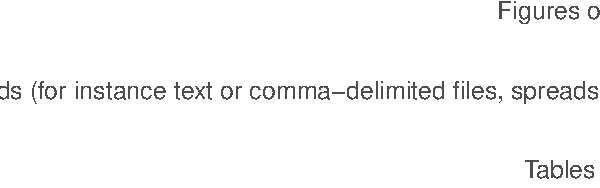
\includegraphics{survey_results_Aug2023_files/figure-latex/dash_delivery-1.pdf}

\hypertarget{characteristics-of-respondents}{%
\subsubsection{6. Characteristics of
respondents}\label{characteristics-of-respondents}}

Finally, the survey requested demographic information from respondents.
This helps the project team get a better understanding of the
dashboard's target audience.

\hypertarget{age-and-gender}{%
\paragraph{6.1 Age and gender}\label{age-and-gender}}

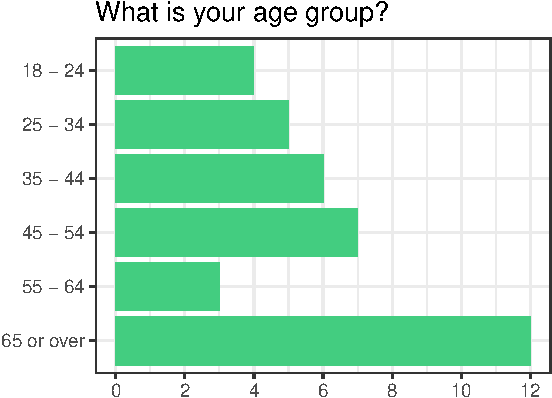
\includegraphics{survey_results_Aug2023_files/figure-latex/age-1.pdf}

\hypertarget{distance-from-the-gtm}{%
\paragraph{6.2 Distance from the GTM}\label{distance-from-the-gtm}}

\begin{verbatim}
## Warning in grid.Call(C_textBounds, as.graphicsAnnot(x$label), x$x, x$y, :
## conversion failure on '31 – 60 minutes' in 'mbcsToSbcs': dot substituted for
## <e2>
\end{verbatim}

\begin{verbatim}
## Warning in grid.Call(C_textBounds, as.graphicsAnnot(x$label), x$x, x$y, :
## conversion failure on '31 – 60 minutes' in 'mbcsToSbcs': dot substituted for
## <80>
\end{verbatim}

\begin{verbatim}
## Warning in grid.Call(C_textBounds, as.graphicsAnnot(x$label), x$x, x$y, :
## conversion failure on '31 – 60 minutes' in 'mbcsToSbcs': dot substituted for
## <93>
\end{verbatim}

\begin{verbatim}
## Warning in grid.Call(C_textBounds, as.graphicsAnnot(x$label), x$x, x$y, :
## conversion failure on '31 – 60 minutes' in 'mbcsToSbcs': dot substituted for
## <e2>
\end{verbatim}

\begin{verbatim}
## Warning in grid.Call(C_textBounds, as.graphicsAnnot(x$label), x$x, x$y, :
## conversion failure on '31 – 60 minutes' in 'mbcsToSbcs': dot substituted for
## <80>
\end{verbatim}

\begin{verbatim}
## Warning in grid.Call(C_textBounds, as.graphicsAnnot(x$label), x$x, x$y, :
## conversion failure on '31 – 60 minutes' in 'mbcsToSbcs': dot substituted for
## <93>
\end{verbatim}

\begin{verbatim}
## Warning in grid.Call(C_textBounds, as.graphicsAnnot(x$label), x$x, x$y, :
## conversion failure on '31 – 60 minutes' in 'mbcsToSbcs': dot substituted for
## <e2>
\end{verbatim}

\begin{verbatim}
## Warning in grid.Call(C_textBounds, as.graphicsAnnot(x$label), x$x, x$y, :
## conversion failure on '31 – 60 minutes' in 'mbcsToSbcs': dot substituted for
## <80>
\end{verbatim}

\begin{verbatim}
## Warning in grid.Call(C_textBounds, as.graphicsAnnot(x$label), x$x, x$y, :
## conversion failure on '31 – 60 minutes' in 'mbcsToSbcs': dot substituted for
## <93>
\end{verbatim}

\begin{verbatim}
## Warning in grid.Call(C_textBounds, as.graphicsAnnot(x$label), x$x, x$y, :
## conversion failure on '31 – 60 minutes' in 'mbcsToSbcs': dot substituted for
## <e2>
\end{verbatim}

\begin{verbatim}
## Warning in grid.Call(C_textBounds, as.graphicsAnnot(x$label), x$x, x$y, :
## conversion failure on '31 – 60 minutes' in 'mbcsToSbcs': dot substituted for
## <80>
\end{verbatim}

\begin{verbatim}
## Warning in grid.Call(C_textBounds, as.graphicsAnnot(x$label), x$x, x$y, :
## conversion failure on '31 – 60 minutes' in 'mbcsToSbcs': dot substituted for
## <93>
\end{verbatim}

\begin{verbatim}
## Warning in grid.Call(C_textBounds, as.graphicsAnnot(x$label), x$x, x$y, :
## conversion failure on '31 – 60 minutes' in 'mbcsToSbcs': dot substituted for
## <e2>
\end{verbatim}

\begin{verbatim}
## Warning in grid.Call(C_textBounds, as.graphicsAnnot(x$label), x$x, x$y, :
## conversion failure on '31 – 60 minutes' in 'mbcsToSbcs': dot substituted for
## <80>
\end{verbatim}

\begin{verbatim}
## Warning in grid.Call(C_textBounds, as.graphicsAnnot(x$label), x$x, x$y, :
## conversion failure on '31 – 60 minutes' in 'mbcsToSbcs': dot substituted for
## <93>
\end{verbatim}

\begin{verbatim}
## Warning in grid.Call(C_textBounds, as.graphicsAnnot(x$label), x$x, x$y, :
## conversion failure on '31 – 60 minutes' in 'mbcsToSbcs': dot substituted for
## <e2>
\end{verbatim}

\begin{verbatim}
## Warning in grid.Call(C_textBounds, as.graphicsAnnot(x$label), x$x, x$y, :
## conversion failure on '31 – 60 minutes' in 'mbcsToSbcs': dot substituted for
## <80>
\end{verbatim}

\begin{verbatim}
## Warning in grid.Call(C_textBounds, as.graphicsAnnot(x$label), x$x, x$y, :
## conversion failure on '31 – 60 minutes' in 'mbcsToSbcs': dot substituted for
## <93>
\end{verbatim}

\begin{verbatim}
## Warning in grid.Call(C_textBounds, as.graphicsAnnot(x$label), x$x, x$y, :
## conversion failure on '31 – 60 minutes' in 'mbcsToSbcs': dot substituted for
## <e2>
\end{verbatim}

\begin{verbatim}
## Warning in grid.Call(C_textBounds, as.graphicsAnnot(x$label), x$x, x$y, :
## conversion failure on '31 – 60 minutes' in 'mbcsToSbcs': dot substituted for
## <80>
\end{verbatim}

\begin{verbatim}
## Warning in grid.Call(C_textBounds, as.graphicsAnnot(x$label), x$x, x$y, :
## conversion failure on '31 – 60 minutes' in 'mbcsToSbcs': dot substituted for
## <93>
\end{verbatim}

\begin{verbatim}
## Warning in grid.Call(C_textBounds, as.graphicsAnnot(x$label), x$x, x$y, :
## conversion failure on '31 – 60 minutes' in 'mbcsToSbcs': dot substituted for
## <e2>
\end{verbatim}

\begin{verbatim}
## Warning in grid.Call(C_textBounds, as.graphicsAnnot(x$label), x$x, x$y, :
## conversion failure on '31 – 60 minutes' in 'mbcsToSbcs': dot substituted for
## <80>
\end{verbatim}

\begin{verbatim}
## Warning in grid.Call(C_textBounds, as.graphicsAnnot(x$label), x$x, x$y, :
## conversion failure on '31 – 60 minutes' in 'mbcsToSbcs': dot substituted for
## <93>
\end{verbatim}

\begin{verbatim}
## Warning in grid.Call(C_textBounds, as.graphicsAnnot(x$label), x$x, x$y, :
## conversion failure on '31 – 60 minutes' in 'mbcsToSbcs': dot substituted for
## <e2>
\end{verbatim}

\begin{verbatim}
## Warning in grid.Call(C_textBounds, as.graphicsAnnot(x$label), x$x, x$y, :
## conversion failure on '31 – 60 minutes' in 'mbcsToSbcs': dot substituted for
## <80>
\end{verbatim}

\begin{verbatim}
## Warning in grid.Call(C_textBounds, as.graphicsAnnot(x$label), x$x, x$y, :
## conversion failure on '31 – 60 minutes' in 'mbcsToSbcs': dot substituted for
## <93>
\end{verbatim}

\begin{verbatim}
## Warning in grid.Call(C_textBounds, as.graphicsAnnot(x$label), x$x, x$y, :
## conversion failure on '31 – 60 minutes' in 'mbcsToSbcs': dot substituted for
## <e2>
\end{verbatim}

\begin{verbatim}
## Warning in grid.Call(C_textBounds, as.graphicsAnnot(x$label), x$x, x$y, :
## conversion failure on '31 – 60 minutes' in 'mbcsToSbcs': dot substituted for
## <80>
\end{verbatim}

\begin{verbatim}
## Warning in grid.Call(C_textBounds, as.graphicsAnnot(x$label), x$x, x$y, :
## conversion failure on '31 – 60 minutes' in 'mbcsToSbcs': dot substituted for
## <93>
\end{verbatim}

\begin{verbatim}
## Warning in grid.Call(C_textBounds, as.graphicsAnnot(x$label), x$x, x$y, :
## conversion failure on '31 – 60 minutes' in 'mbcsToSbcs': dot substituted for
## <e2>
\end{verbatim}

\begin{verbatim}
## Warning in grid.Call(C_textBounds, as.graphicsAnnot(x$label), x$x, x$y, :
## conversion failure on '31 – 60 minutes' in 'mbcsToSbcs': dot substituted for
## <80>
\end{verbatim}

\begin{verbatim}
## Warning in grid.Call(C_textBounds, as.graphicsAnnot(x$label), x$x, x$y, :
## conversion failure on '31 – 60 minutes' in 'mbcsToSbcs': dot substituted for
## <93>
\end{verbatim}

\begin{verbatim}
## Warning in grid.Call(C_textBounds, as.graphicsAnnot(x$label), x$x, x$y, :
## conversion failure on '31 – 60 minutes' in 'mbcsToSbcs': dot substituted for
## <e2>
\end{verbatim}

\begin{verbatim}
## Warning in grid.Call(C_textBounds, as.graphicsAnnot(x$label), x$x, x$y, :
## conversion failure on '31 – 60 minutes' in 'mbcsToSbcs': dot substituted for
## <80>
\end{verbatim}

\begin{verbatim}
## Warning in grid.Call(C_textBounds, as.graphicsAnnot(x$label), x$x, x$y, :
## conversion failure on '31 – 60 minutes' in 'mbcsToSbcs': dot substituted for
## <93>
\end{verbatim}

\begin{verbatim}
## Warning in grid.Call(C_textBounds, as.graphicsAnnot(x$label), x$x, x$y, :
## conversion failure on '31 – 60 minutes' in 'mbcsToSbcs': dot substituted for
## <e2>
\end{verbatim}

\begin{verbatim}
## Warning in grid.Call(C_textBounds, as.graphicsAnnot(x$label), x$x, x$y, :
## conversion failure on '31 – 60 minutes' in 'mbcsToSbcs': dot substituted for
## <80>
\end{verbatim}

\begin{verbatim}
## Warning in grid.Call(C_textBounds, as.graphicsAnnot(x$label), x$x, x$y, :
## conversion failure on '31 – 60 minutes' in 'mbcsToSbcs': dot substituted for
## <93>
\end{verbatim}

\begin{verbatim}
## Warning in grid.Call(C_textBounds, as.graphicsAnnot(x$label), x$x, x$y, :
## conversion failure on '31 – 60 minutes' in 'mbcsToSbcs': dot substituted for
## <e2>
\end{verbatim}

\begin{verbatim}
## Warning in grid.Call(C_textBounds, as.graphicsAnnot(x$label), x$x, x$y, :
## conversion failure on '31 – 60 minutes' in 'mbcsToSbcs': dot substituted for
## <80>
\end{verbatim}

\begin{verbatim}
## Warning in grid.Call(C_textBounds, as.graphicsAnnot(x$label), x$x, x$y, :
## conversion failure on '31 – 60 minutes' in 'mbcsToSbcs': dot substituted for
## <93>
\end{verbatim}

\begin{verbatim}
## Warning in grid.Call(C_textBounds, as.graphicsAnnot(x$label), x$x, x$y, :
## conversion failure on '31 – 60 minutes' in 'mbcsToSbcs': dot substituted for
## <e2>
\end{verbatim}

\begin{verbatim}
## Warning in grid.Call(C_textBounds, as.graphicsAnnot(x$label), x$x, x$y, :
## conversion failure on '31 – 60 minutes' in 'mbcsToSbcs': dot substituted for
## <80>
\end{verbatim}

\begin{verbatim}
## Warning in grid.Call(C_textBounds, as.graphicsAnnot(x$label), x$x, x$y, :
## conversion failure on '31 – 60 minutes' in 'mbcsToSbcs': dot substituted for
## <93>
\end{verbatim}

\begin{verbatim}
## Warning in grid.Call.graphics(C_text, as.graphicsAnnot(x$label), x$x, x$y, :
## conversion failure on '31 – 60 minutes' in 'mbcsToSbcs': dot substituted for
## <e2>
\end{verbatim}

\begin{verbatim}
## Warning in grid.Call.graphics(C_text, as.graphicsAnnot(x$label), x$x, x$y, :
## conversion failure on '31 – 60 minutes' in 'mbcsToSbcs': dot substituted for
## <80>
\end{verbatim}

\begin{verbatim}
## Warning in grid.Call.graphics(C_text, as.graphicsAnnot(x$label), x$x, x$y, :
## conversion failure on '31 – 60 minutes' in 'mbcsToSbcs': dot substituted for
## <93>
\end{verbatim}

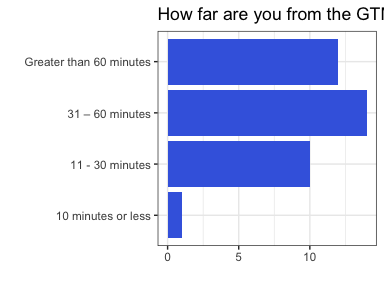
\includegraphics{survey_results_Aug2023_files/figure-latex/distance-1.pdf}

Add professions

\hypertarget{next-steps}{%
\subsection{Next steps}\label{next-steps}}

The project team will still refine details in this report, and
distribute/publish the final version by the end of August 2023. This
final report will also include dashboard design considerations and
recommendations based on the survey results.

If you have suggestions, comments or requests, please email
Dr.~Geraldine Klarenberg at
\href{mailto:gklarenberg@gmail.com}{\nolinkurl{gklarenberg@gmail.com}}.

\hypertarget{appendix-visualizations-accompanying-section-6}{%
\subsection{Appendix: Visualizations accompanying section
6}\label{appendix-visualizations-accompanying-section-6}}

The figures below provide visual interpretations of the table in section
6, on the datasets that respondents have accessed.

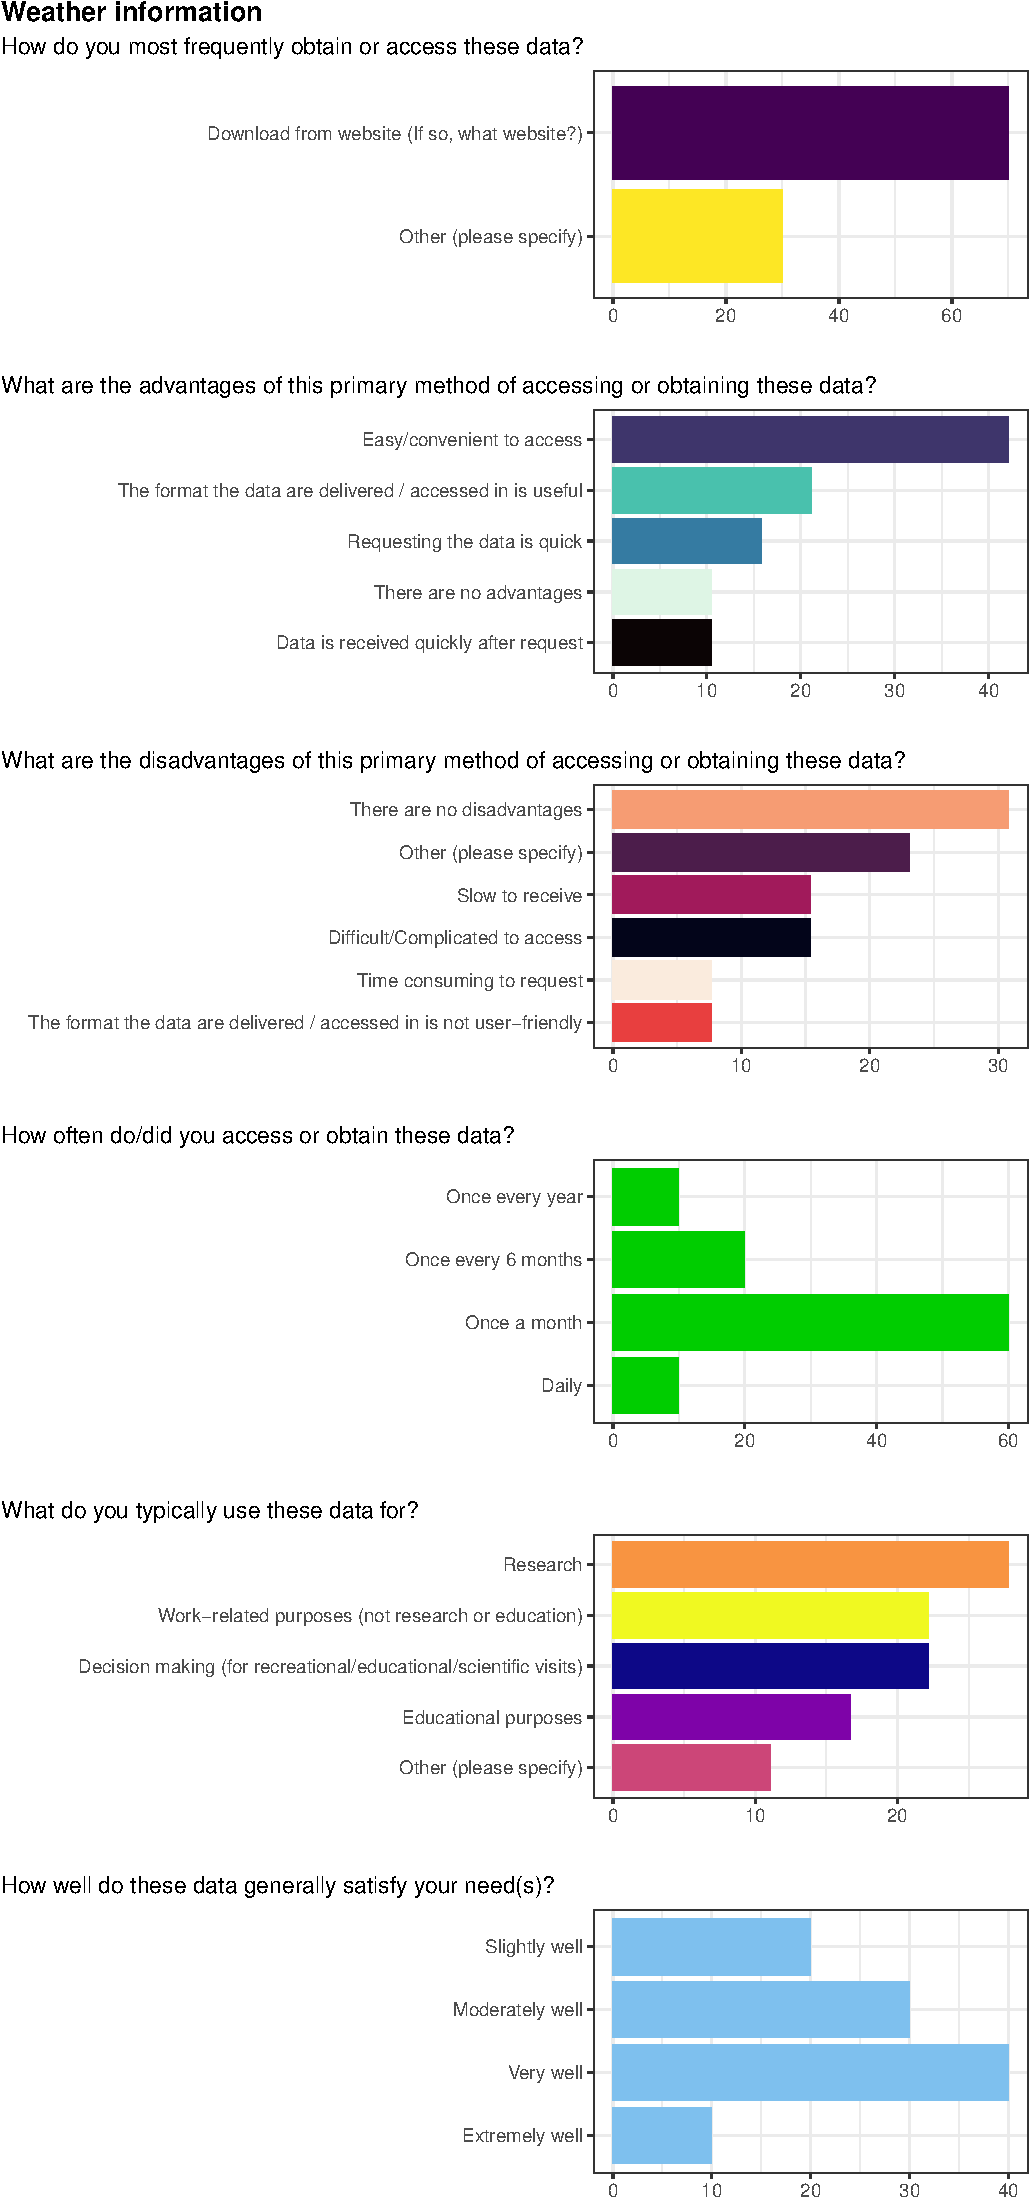
\includegraphics{survey_results_Aug2023_files/figure-latex/all_q_per_dataset-1.pdf}
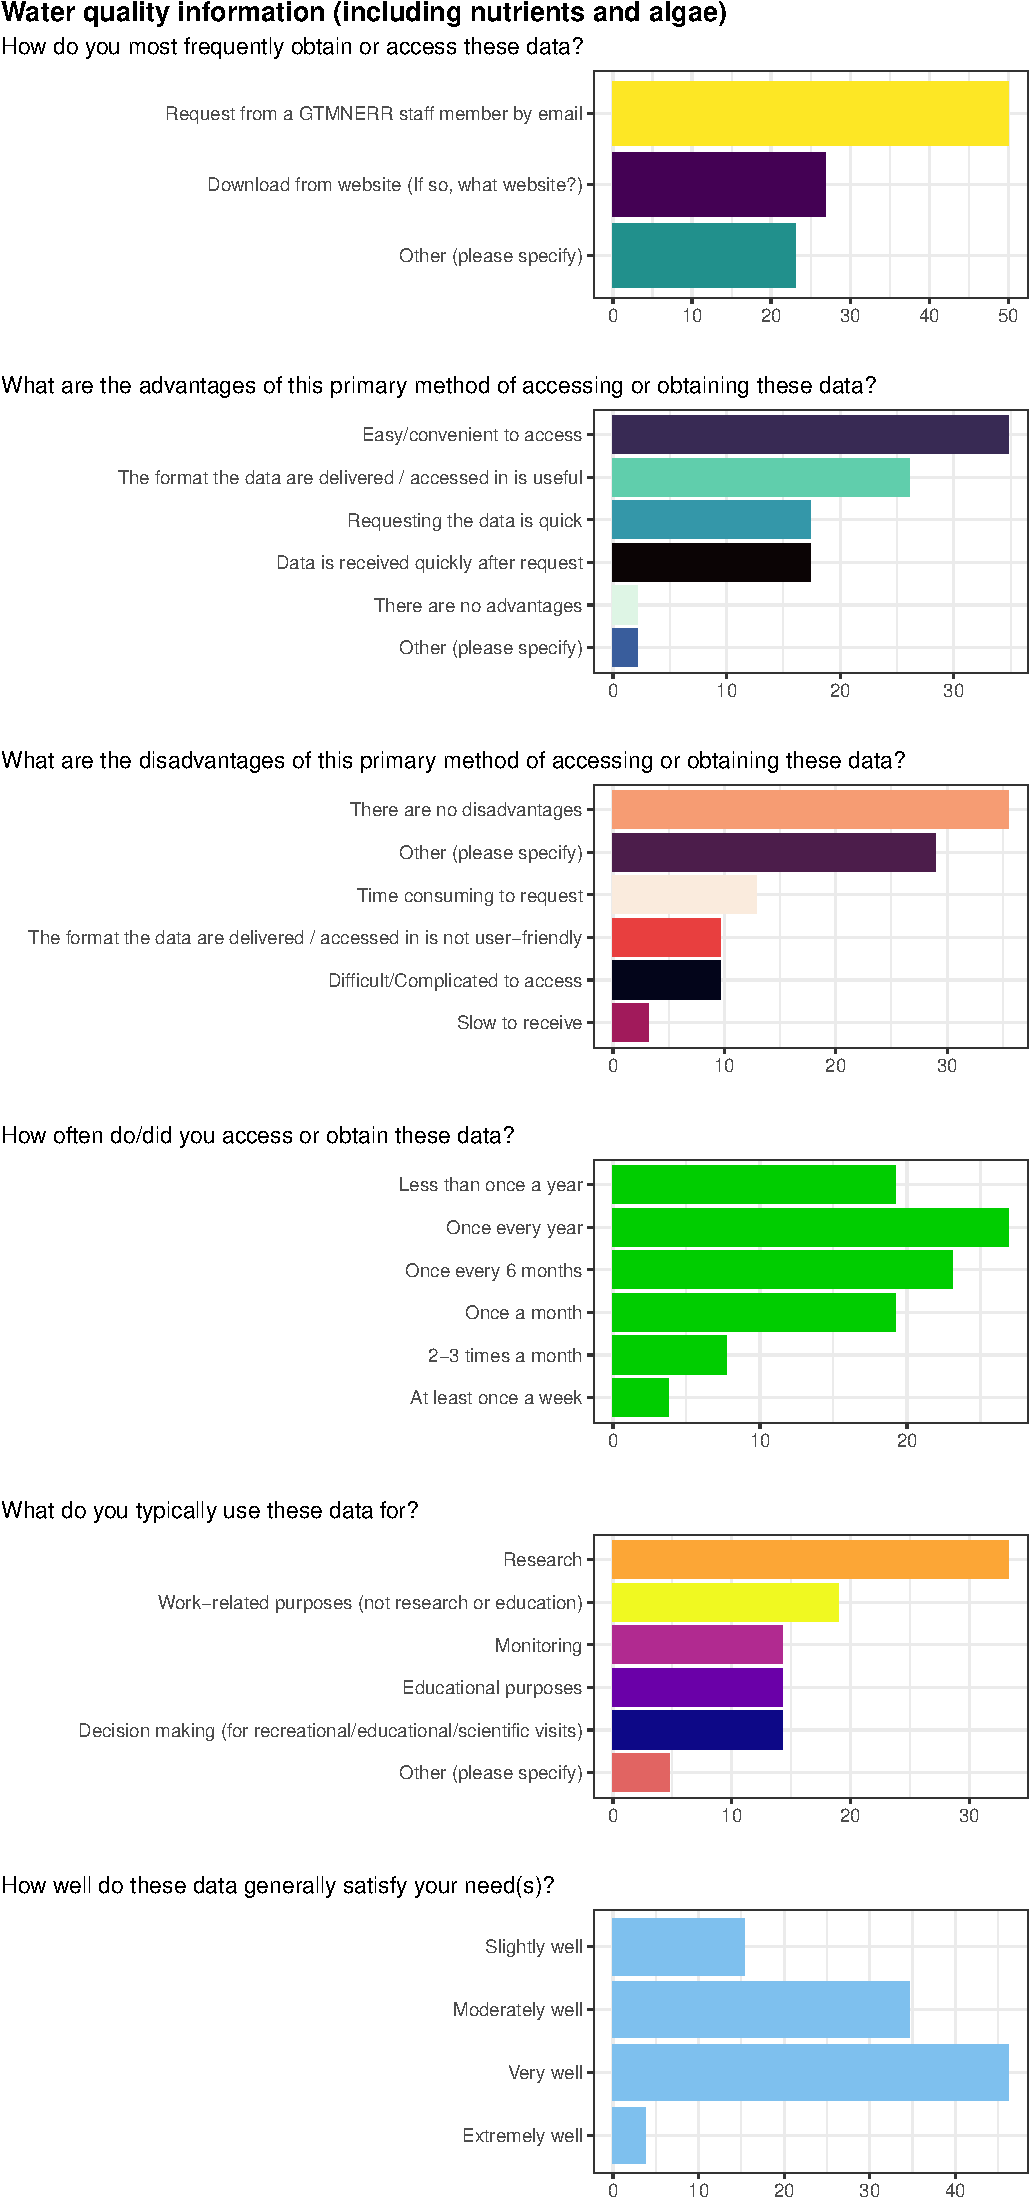
\includegraphics{survey_results_Aug2023_files/figure-latex/all_q_per_dataset-2.pdf}
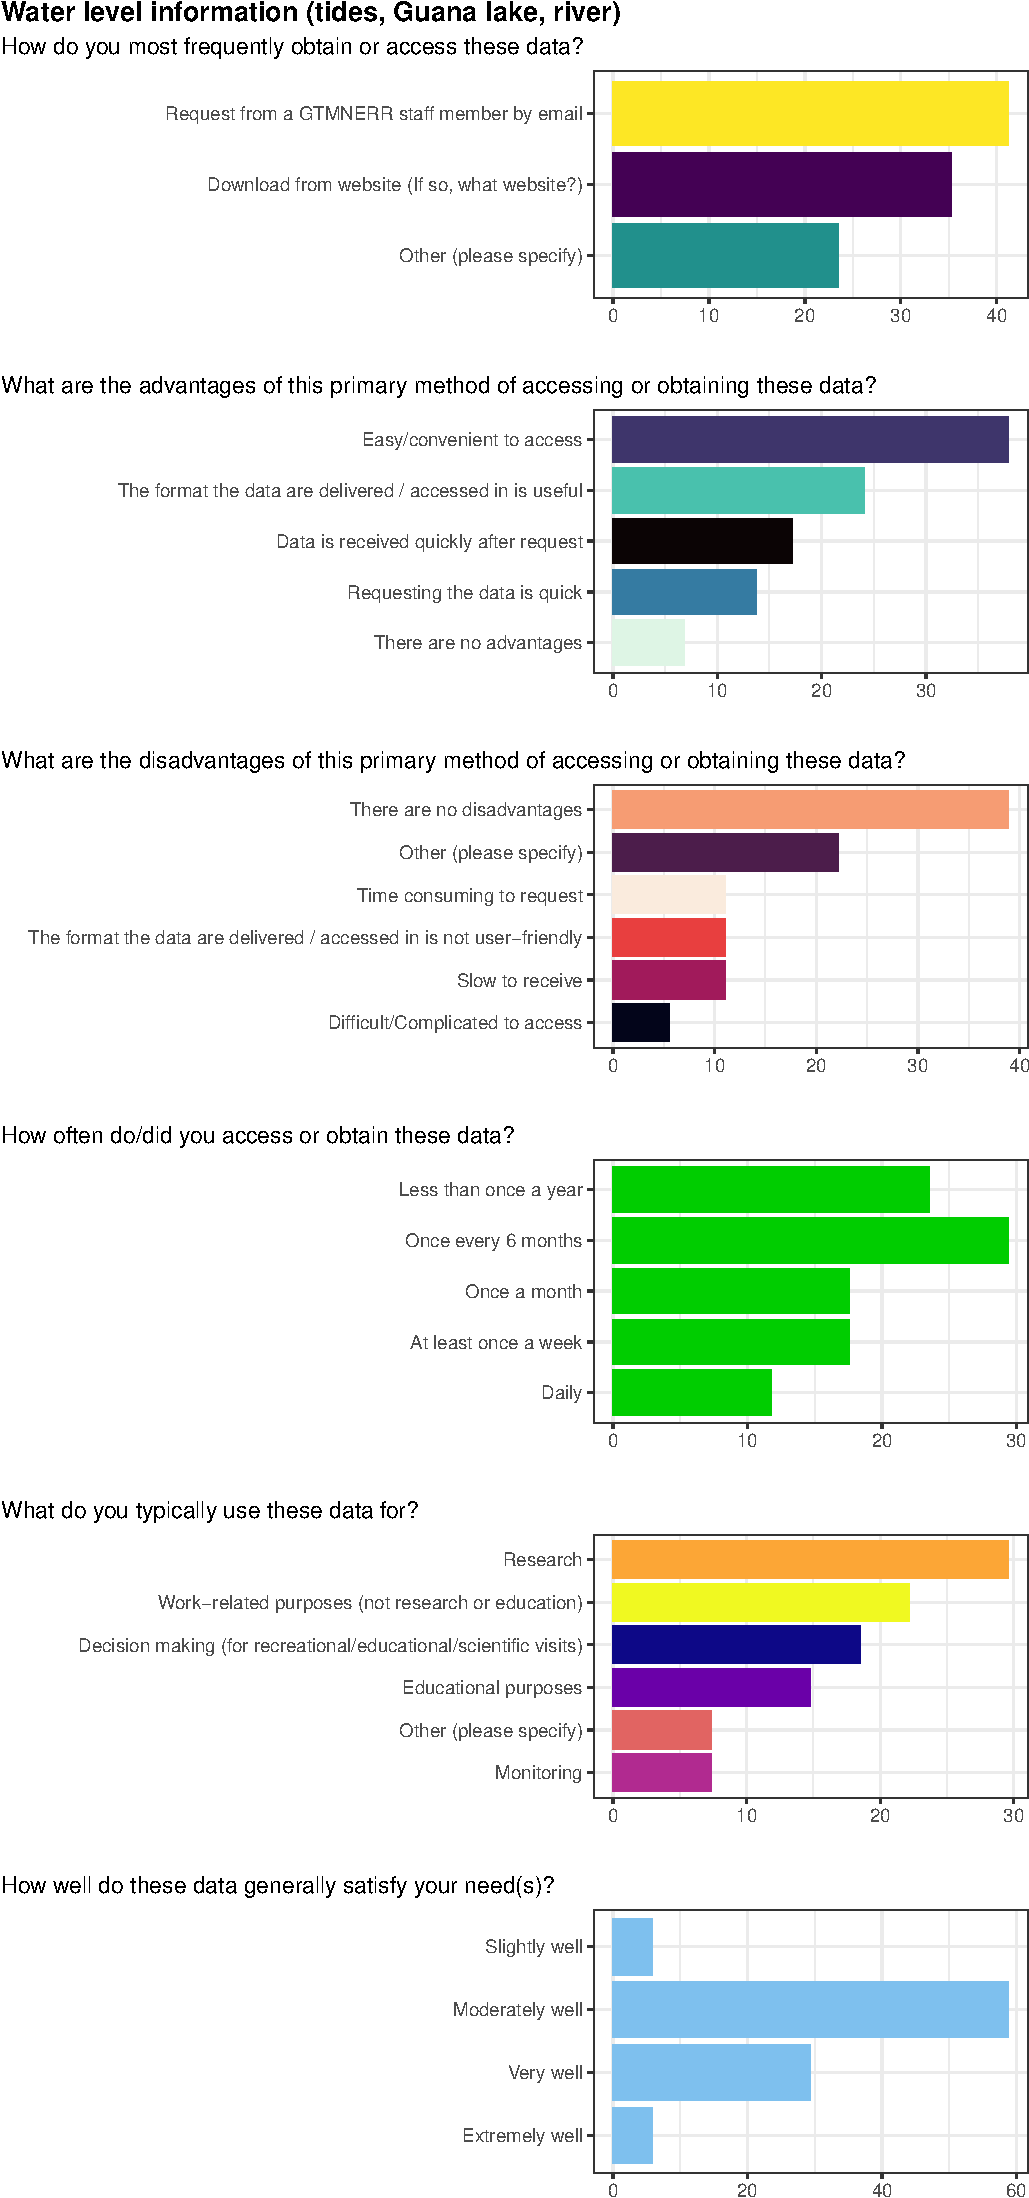
\includegraphics{survey_results_Aug2023_files/figure-latex/all_q_per_dataset-3.pdf}
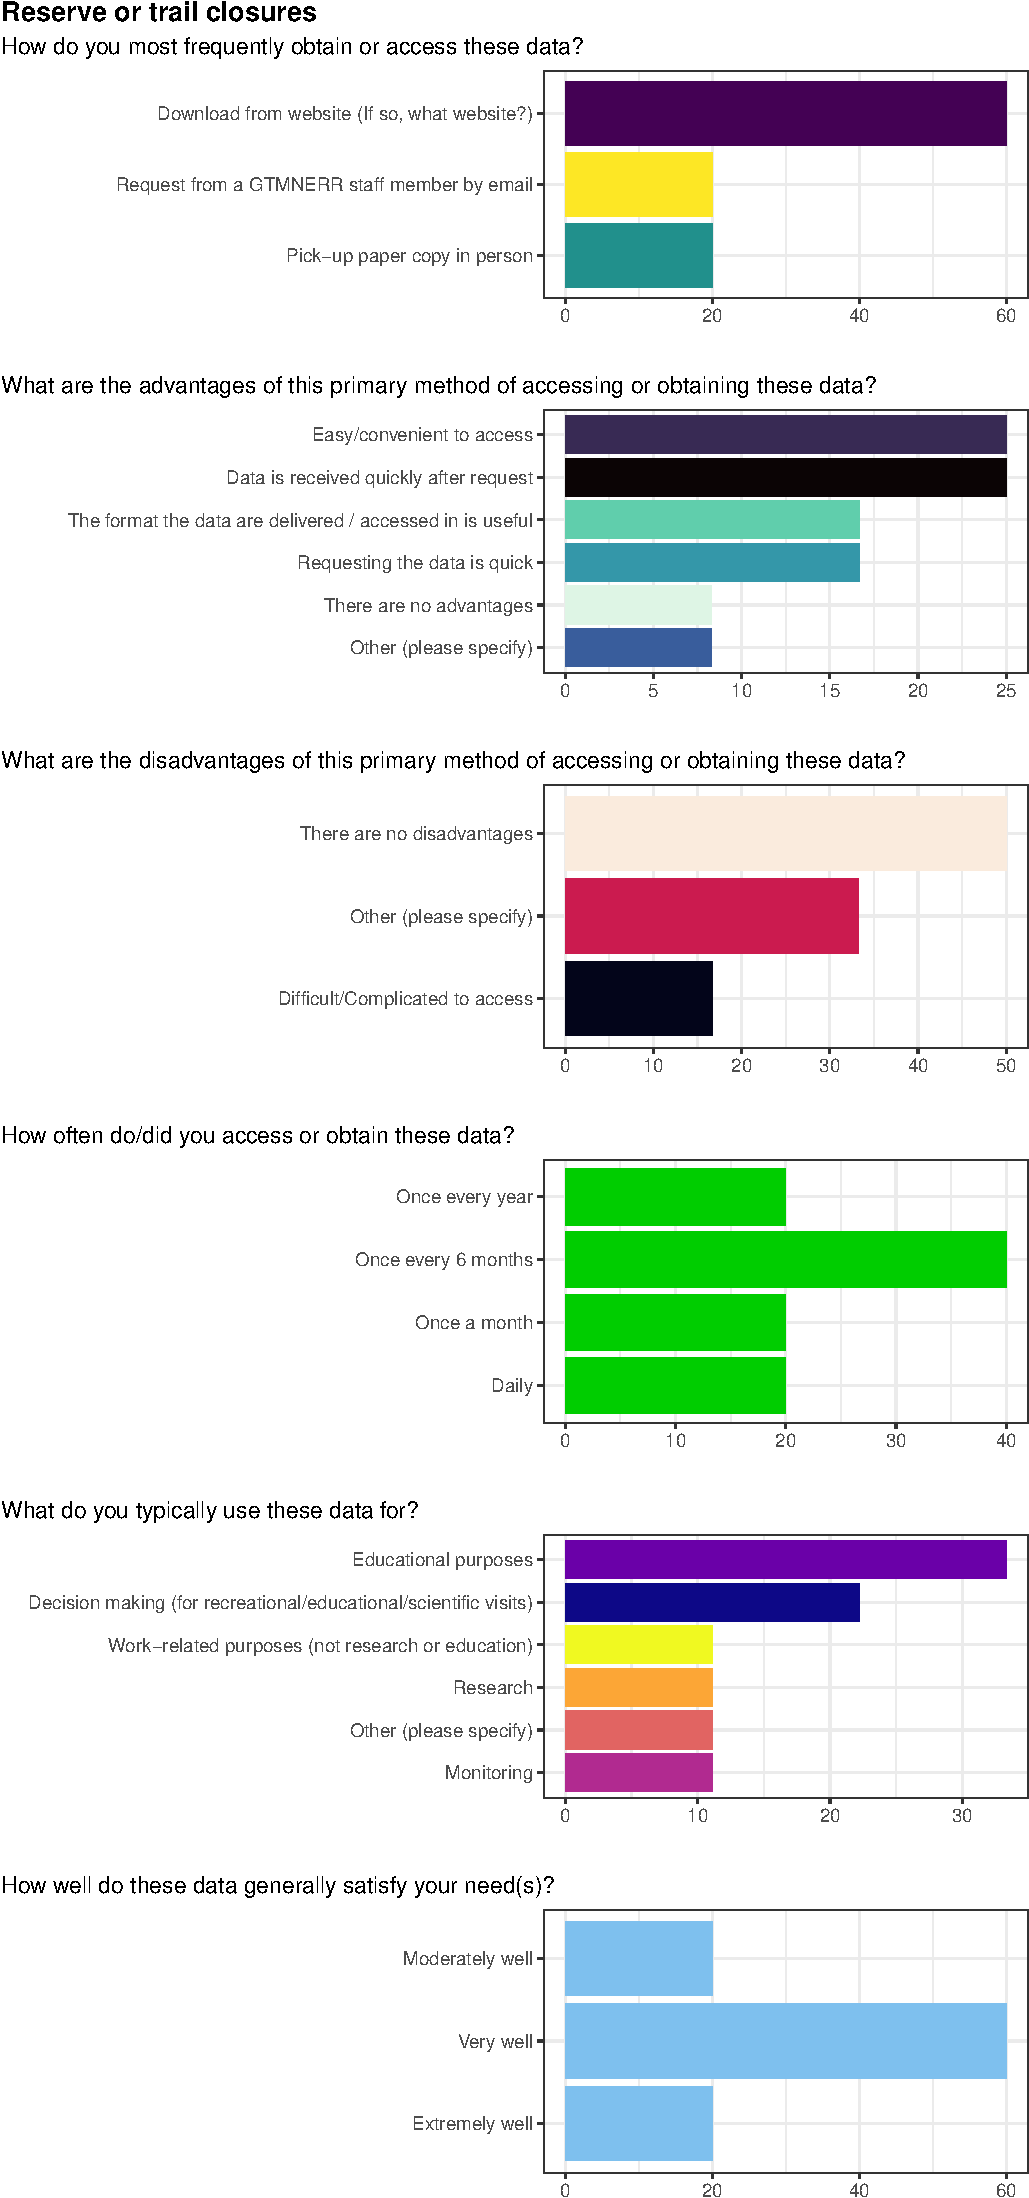
\includegraphics{survey_results_Aug2023_files/figure-latex/all_q_per_dataset-4.pdf}
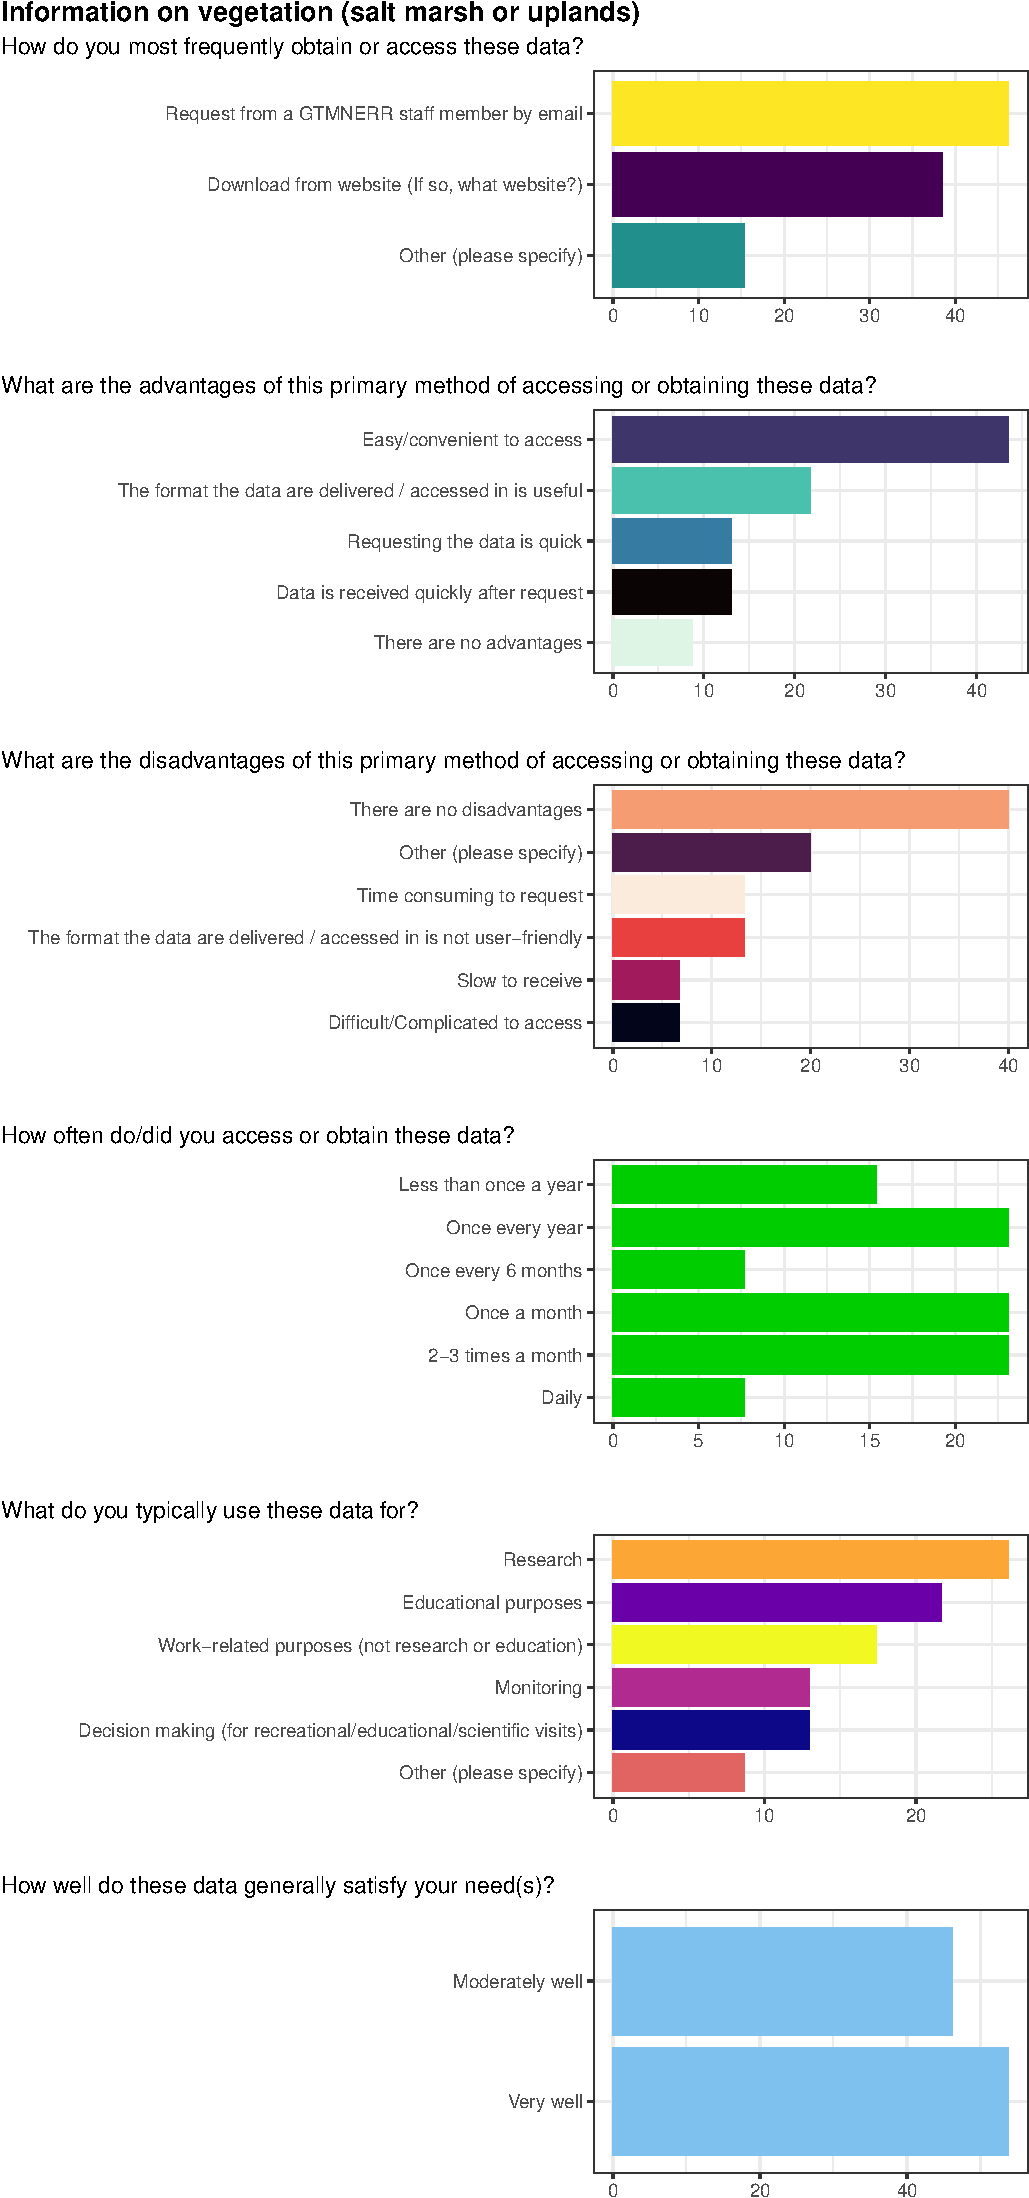
\includegraphics{survey_results_Aug2023_files/figure-latex/all_q_per_dataset-5.pdf}
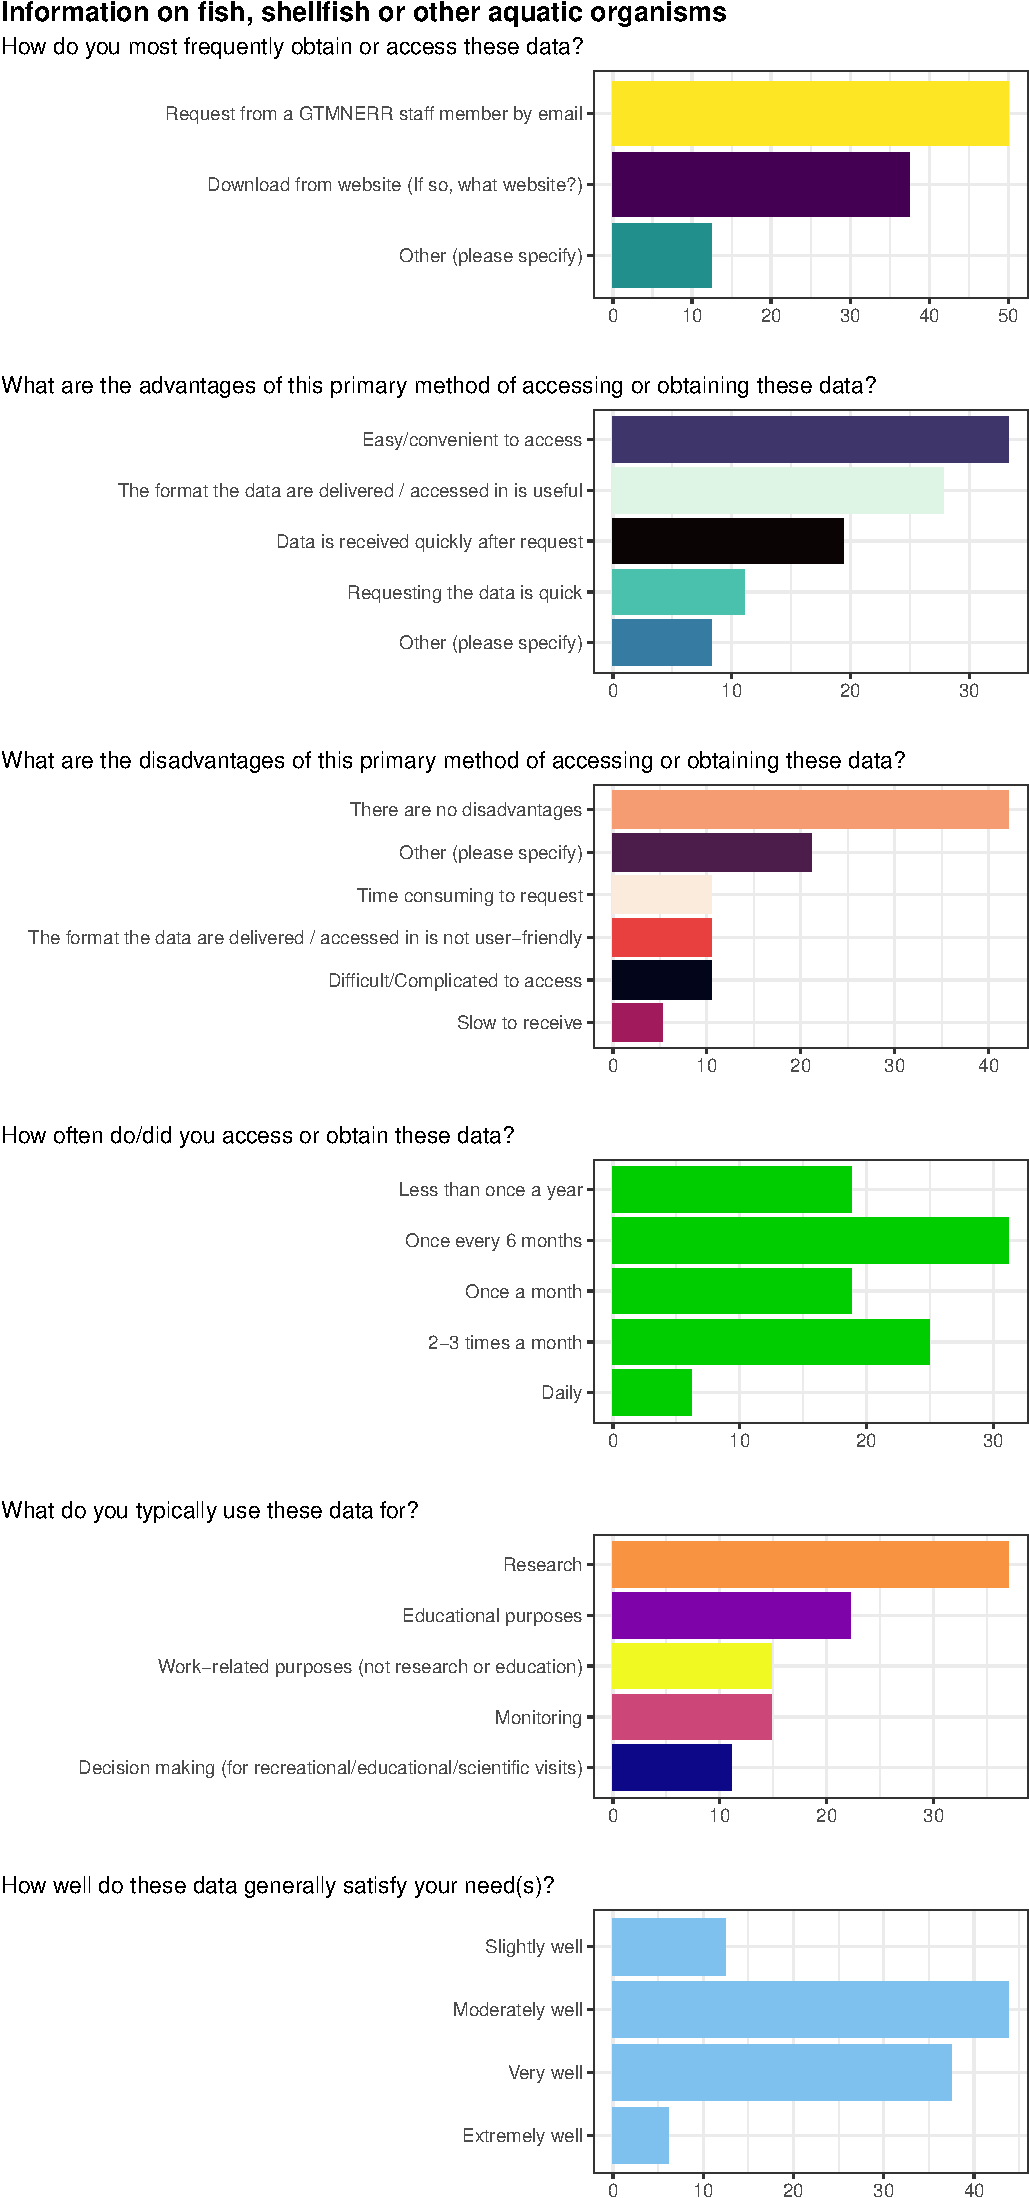
\includegraphics{survey_results_Aug2023_files/figure-latex/all_q_per_dataset-6.pdf}
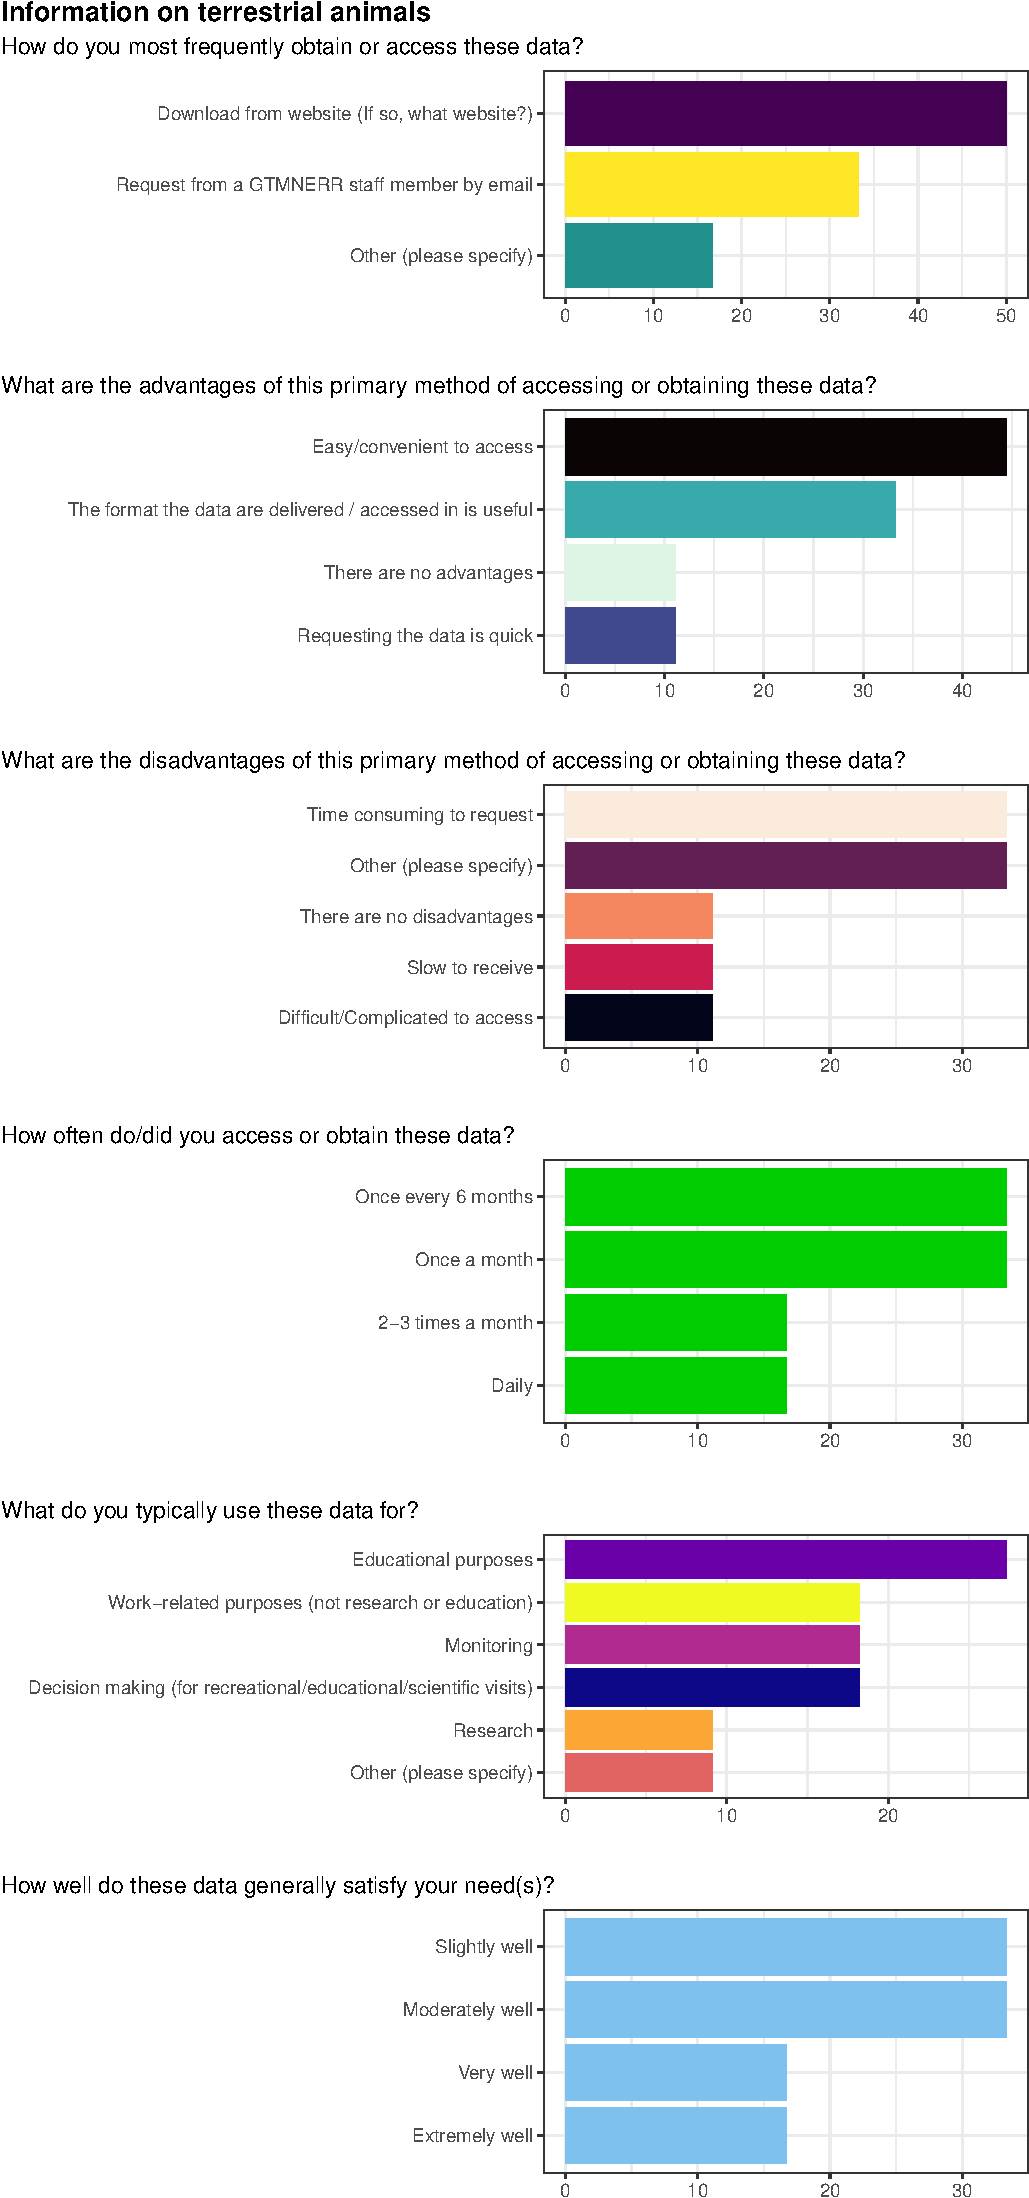
\includegraphics{survey_results_Aug2023_files/figure-latex/all_q_per_dataset-7.pdf}
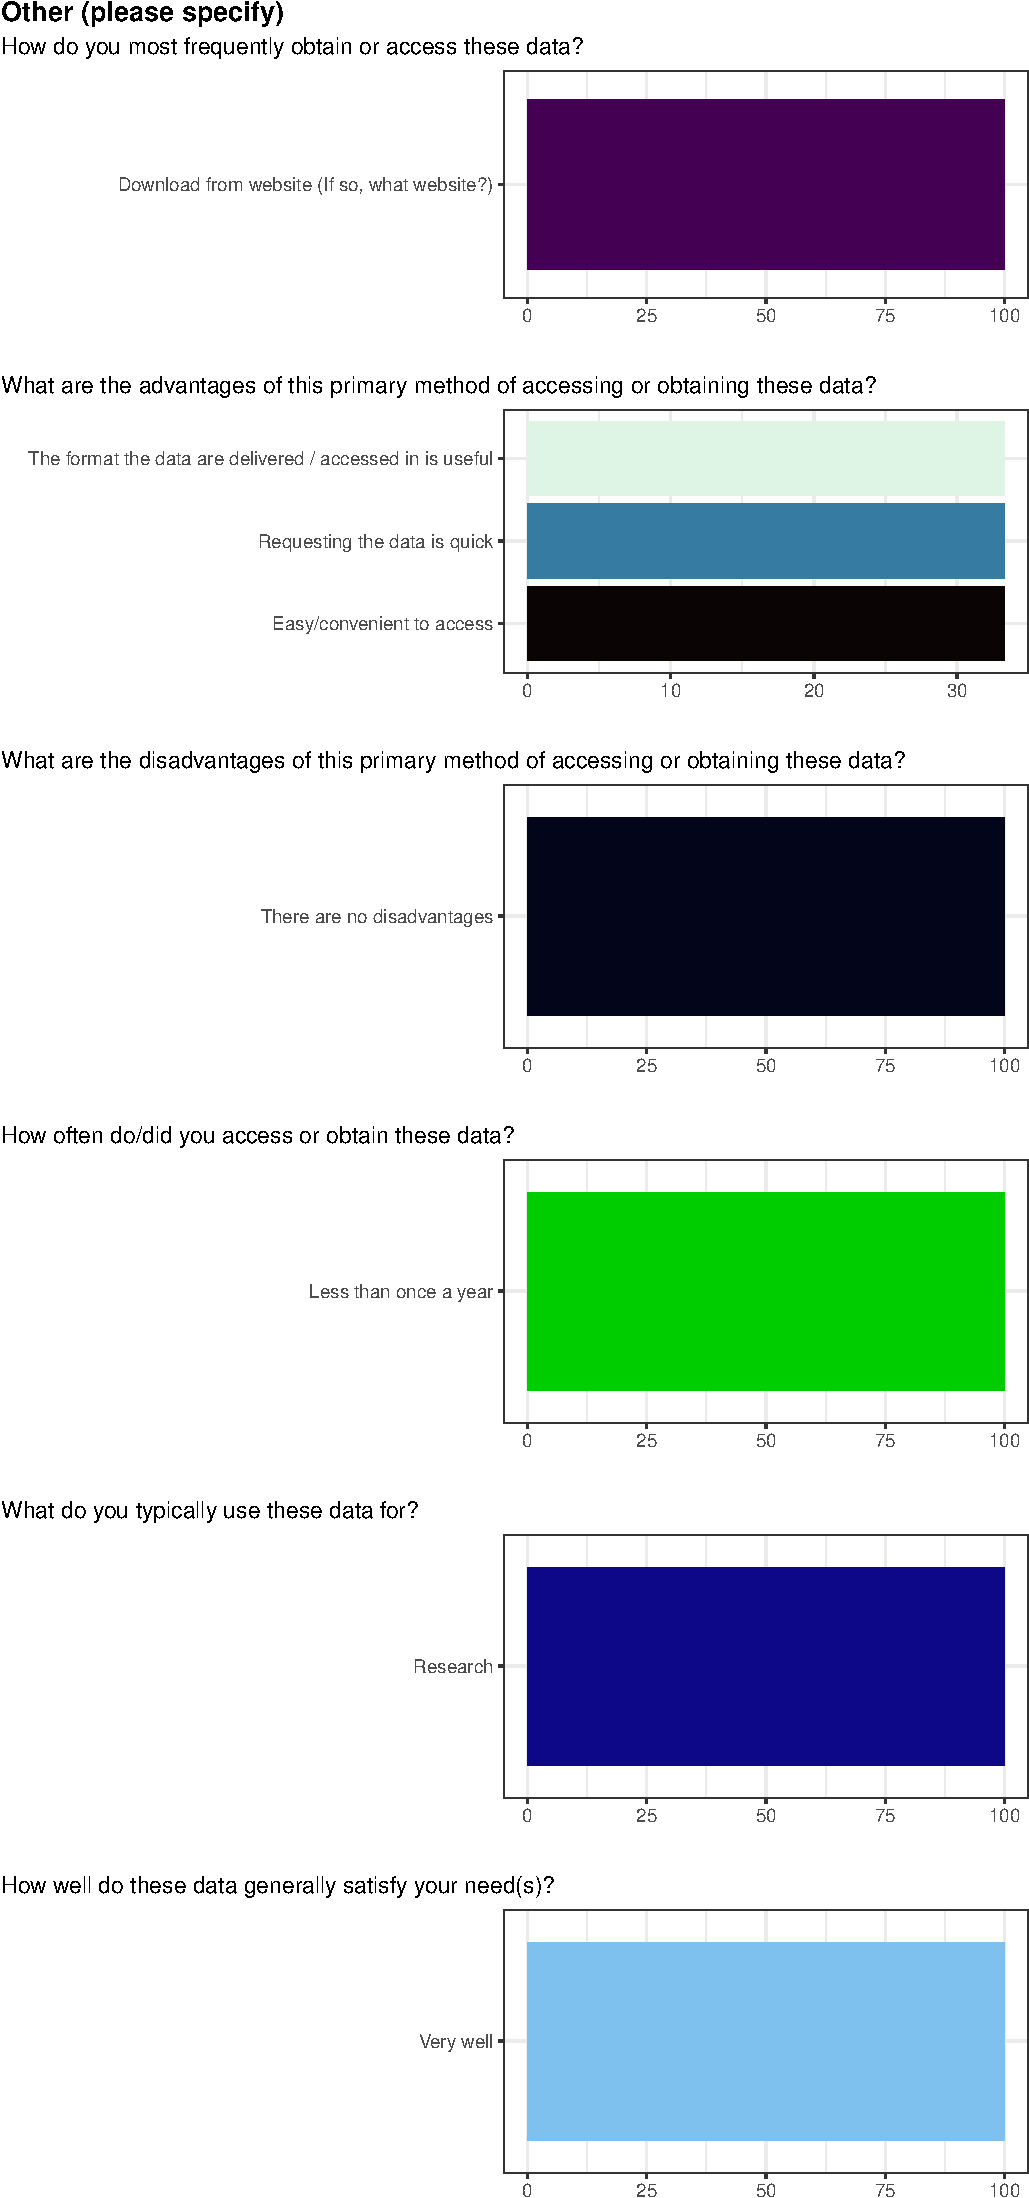
\includegraphics{survey_results_Aug2023_files/figure-latex/all_q_per_dataset-8.pdf}

\end{document}
